
In order to use the substructure tools that have been presented above, 
it is necessary to measure several supporting numbers.
The first is the subjet energy scale. 
%The second is the selection efficiency of the substructure tools in the
%data (compared to the Monte Carlo). The third is the rate at which generic 
%QCD jets fake the selection (the ``mistag rate''). 

\ifnpas
\subsection{Subjet energy scale}
\fi 
\label{sec:substructure_jec}




\ifnpas

The prescription we have followed to correct our jets is to apply the
\verb!AK5PFchs! corrections to our jets. This is not exactly correct
because we are using jets built with different clustering algorithms and different cone size (0.7, 0.8, 1.2).
However, these are the only corrections that are sufficiently commissioned
for usage. There is not expected to be a large difference in response between
these types of jets in a boosted kinematical regime.

Figure~\ref{figs:ptRatio} 
shows the comparison of the reconstructed jet momentum (corrected to {\tt L1FastJet, L2Relative, L3Absolute}) scale and 
resolution by comparing to the generator level jets for AK5, AK7 and AK8 generator level jets, where the  generator
level jets have no substructure
algorithms applied. This means that in each plot the ungroomed distributions show the scale and resolution for AK5, AK7 and AK8 jet compared to the matching same radius generator jets, while for the groomed jets we use the same ungroomed ``denominator''.  
The scale and resolution are obtained by ``slicing'' the jet $p_T$ or pseudorapidity distributions and performing gaussian fits of the reconstructed/generated ratio distributions. We then report the mean (scale offset) and sigma (resolution) from these fits as a function of the jet $p_T$ or pseudorapidity.
  
We can notice that the response for filtered jet is the closest to the ungroomed jets response (always within less than 5\%). 
The response becomes reasonably flat in the boosted regime above 200-250 GeV, apart for the pruned jets (and in a less evident way for the trimmed). 
The jet pruning and trimming (intentionally) removes part
of the jet, and that fraction is larger at lower momenta. If one compares the
response of jet-pruned reconstructed jets with respect to unpruned
generator-level jets, a large difference is seen at low $\pt$ (maximally 8\%).
 
\begin{figure}[!htb]
\centering
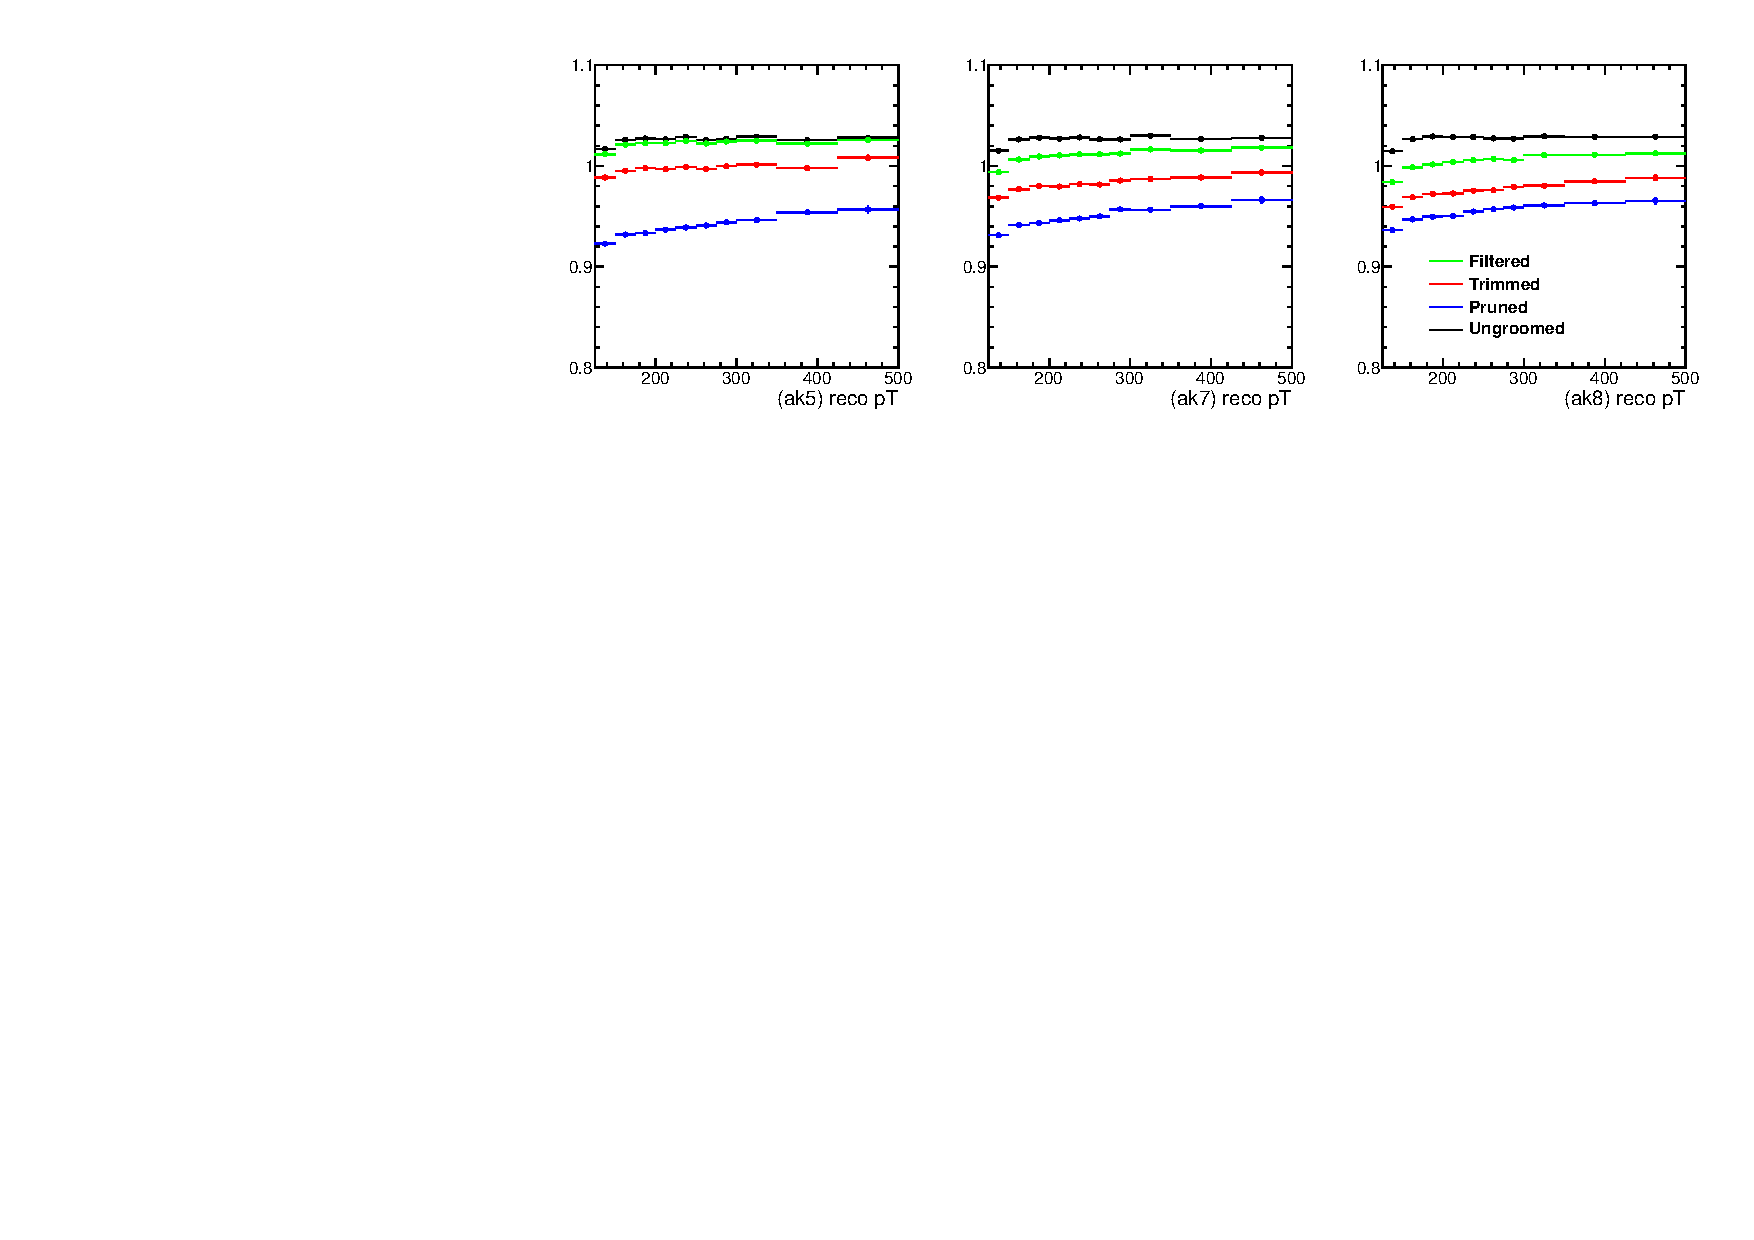
\includegraphics[width=1.0\textwidth]{figs/ptRatioVsPt_mean.pdf}
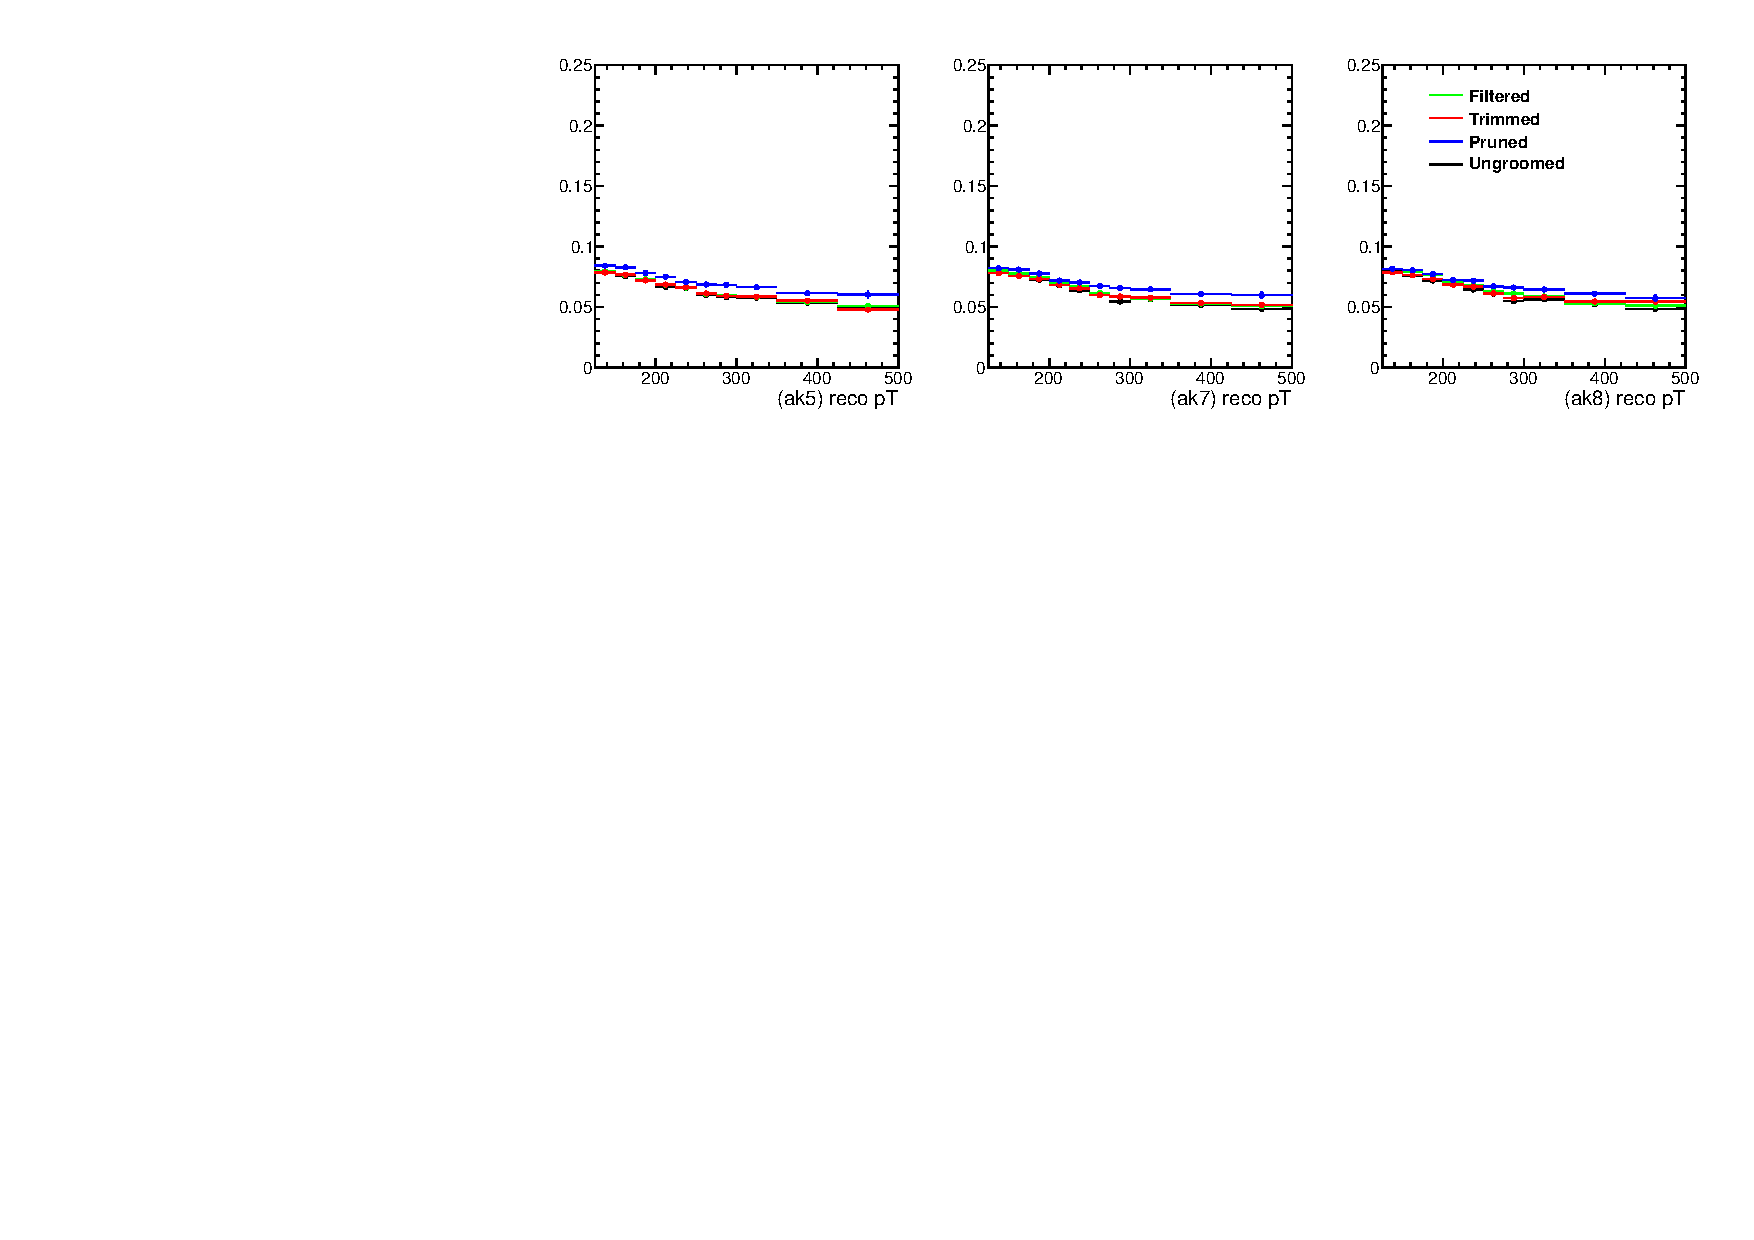
\includegraphics[width=1.0\textwidth]{figs/ptRatioVsPt_sigma.pdf}
\caption{Jet response (top: scale offset, bottom: resolution) for different jet algorithms as a function of the jet momentum. Here, the
  substructure algorithms are compared to the
  generator-level AK5, AK7 and AK8 jets without the substructure algorithms applied.}
\label{figs:ptRatio}
\end{figure}


Figure~\ref{figs:ptRatiovsEta} shows the corresponding distributions as a function of the ungroomed generated jet pseudorapidity. The noticeable behaviour in the groomed jets is a residual dependence in the resolution in the forward region, that becomes more and more pronounced the more aggressive the grooming is. Most likely, the effect, around 2\%, is due to a residual clustering dependence that is not present in the ungroomed jet corrections.  
Figure~\ref{figs:ptRatiovsPV} shows the jet momentum resolution as a function of the primary vertex multiplicity, and it shows the same PU dependency for groomned and ungroomed jets.  
 

%\includegraphics[width=1.0\textwidth]{figs/ak5ca8compare_genunpruned_jetResAvg}
%\caption{Jet response for different jet algorithms. Here, the
%  substructure algorithms are compared to the unmodified
%  generator-level jets ({\tt AK5GenJets} and {\tt CA8GenJets} for
%  the AK5 and CA8 algorithms, respectively).}
%\label{figs:ak5ca8compare_genunpruned_jetResAvg}
%\end{figure}


\begin{figure}[htb]
\centering
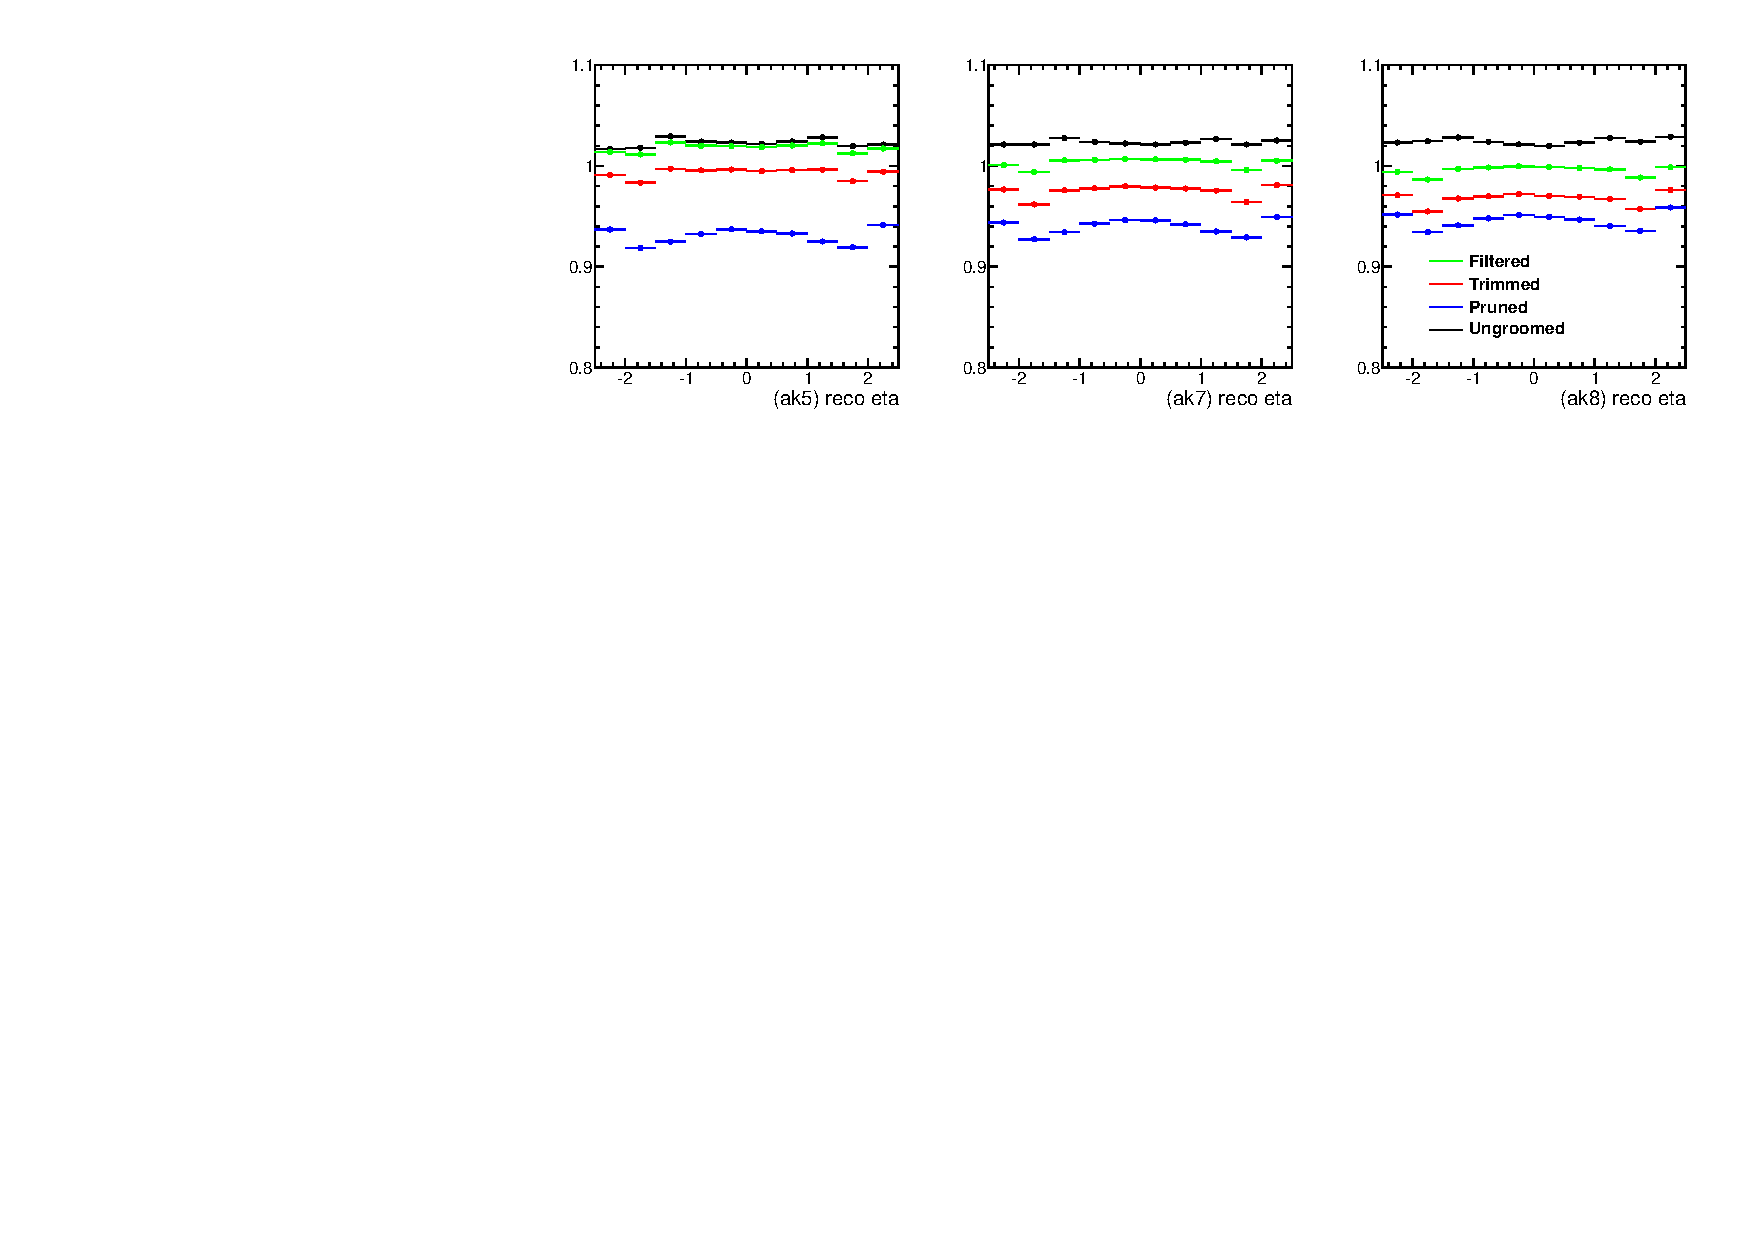
\includegraphics[width=1.0\textwidth]{figs/ptRatioVsEta_mean.pdf}
\caption{Jet response for different jet algorithms as a function of the jet pseudorapidity. Here, the
  substructure algorithms are compared to the
  generator-level AK5, AK7 and AK8 jets without the substructure algorithms applied.}
\label{figs:ptRatiovsEta}
\end{figure}

\begin{figure}[htb]
\centering
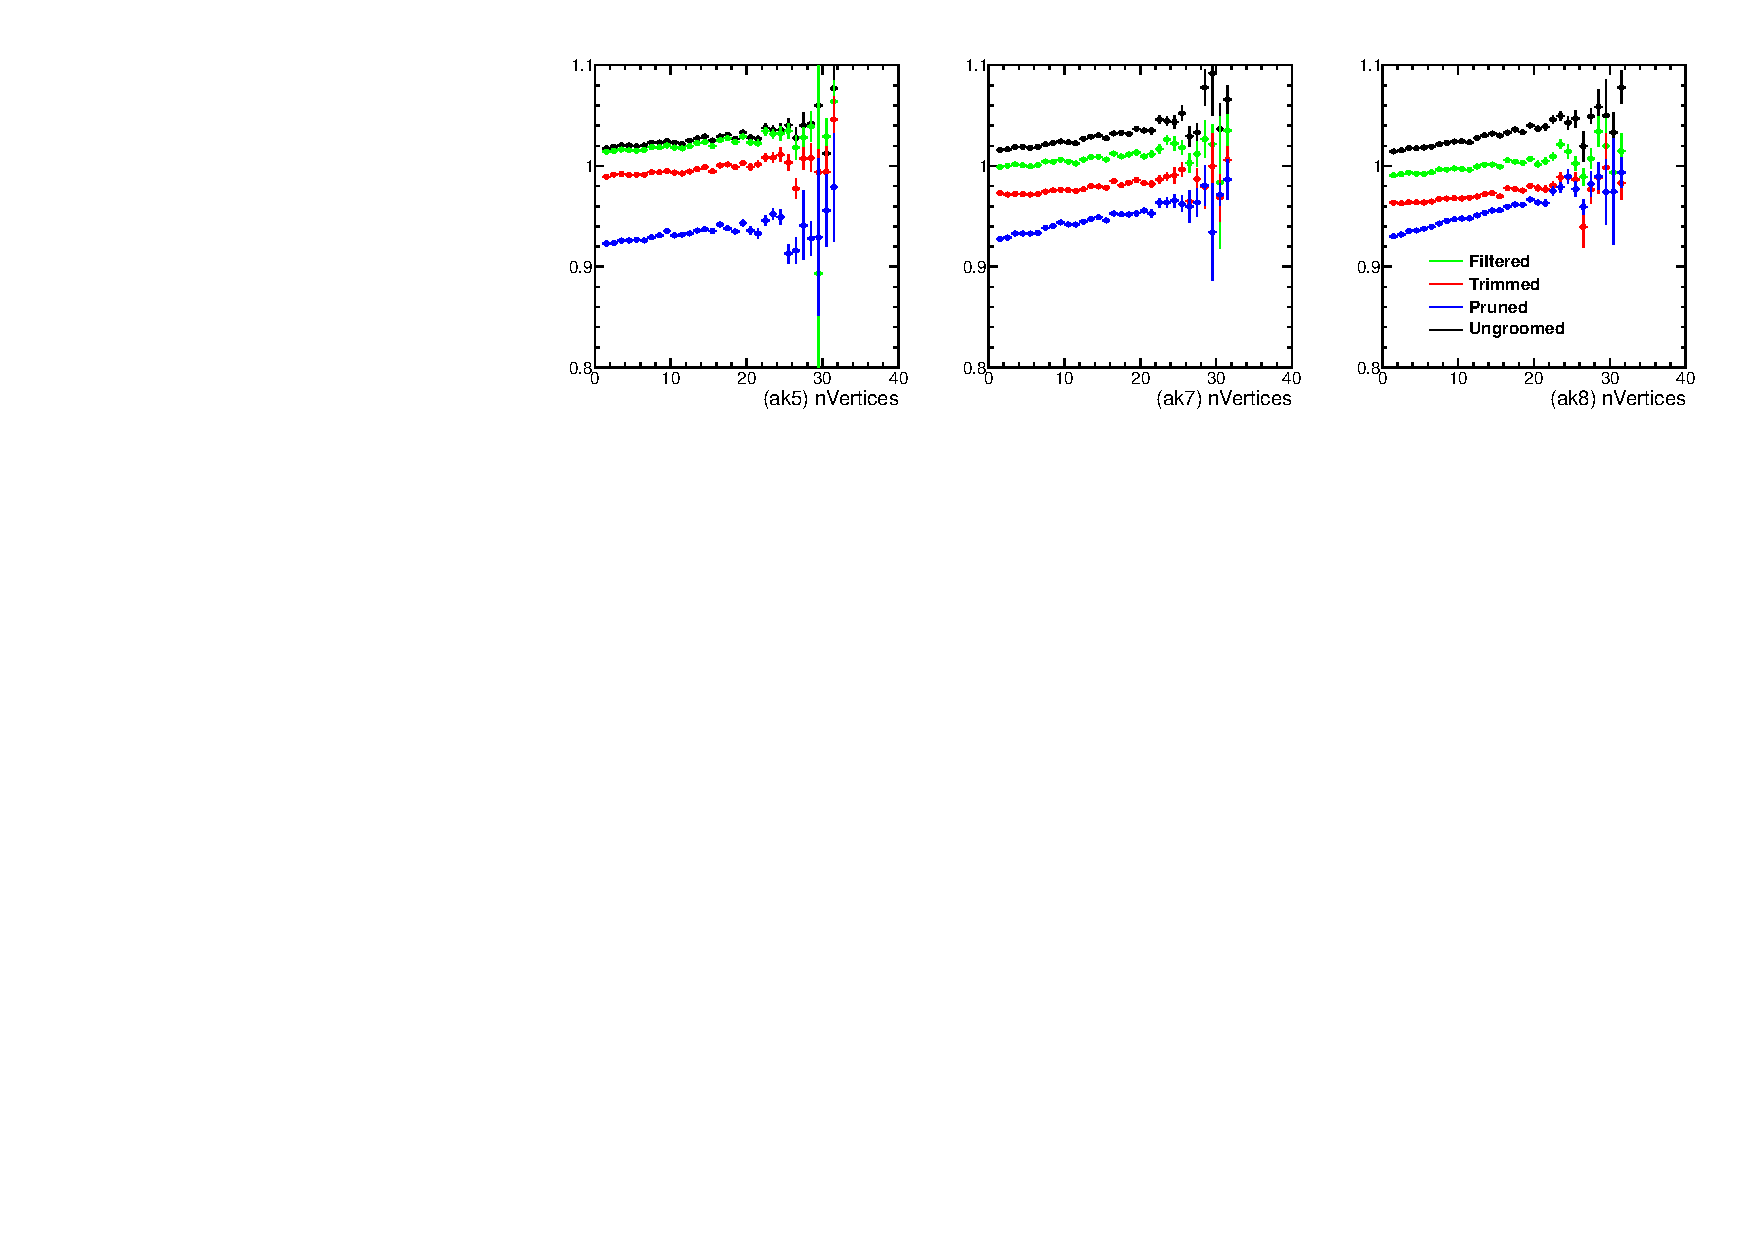
\includegraphics[width=1.0\textwidth]{figs/ptRatioVsNV_mean.pdf}
\caption{Jet response for different jet algorithms as a function of the primary vertex multiplicity in the event. Here, the
  substructure algorithms are compared to the
  generator-level AK5, AK7 and AK8 jets without the substructure algorithms applied.}
\label{figs:ptRatiovsPV}
\end{figure}


We then look at the corresponding resolution study for the jet mass. We first show the mass ratio dependence versus the jet momentum. Fig.~\ref{figs:massRatio} shows the ratio of the reconstructed  (ungroomed or groomed) jet mass over the ungrooomed generator  AK5, AK7 and AK8 jets. 

\begin{figure}[!htb]
\centering
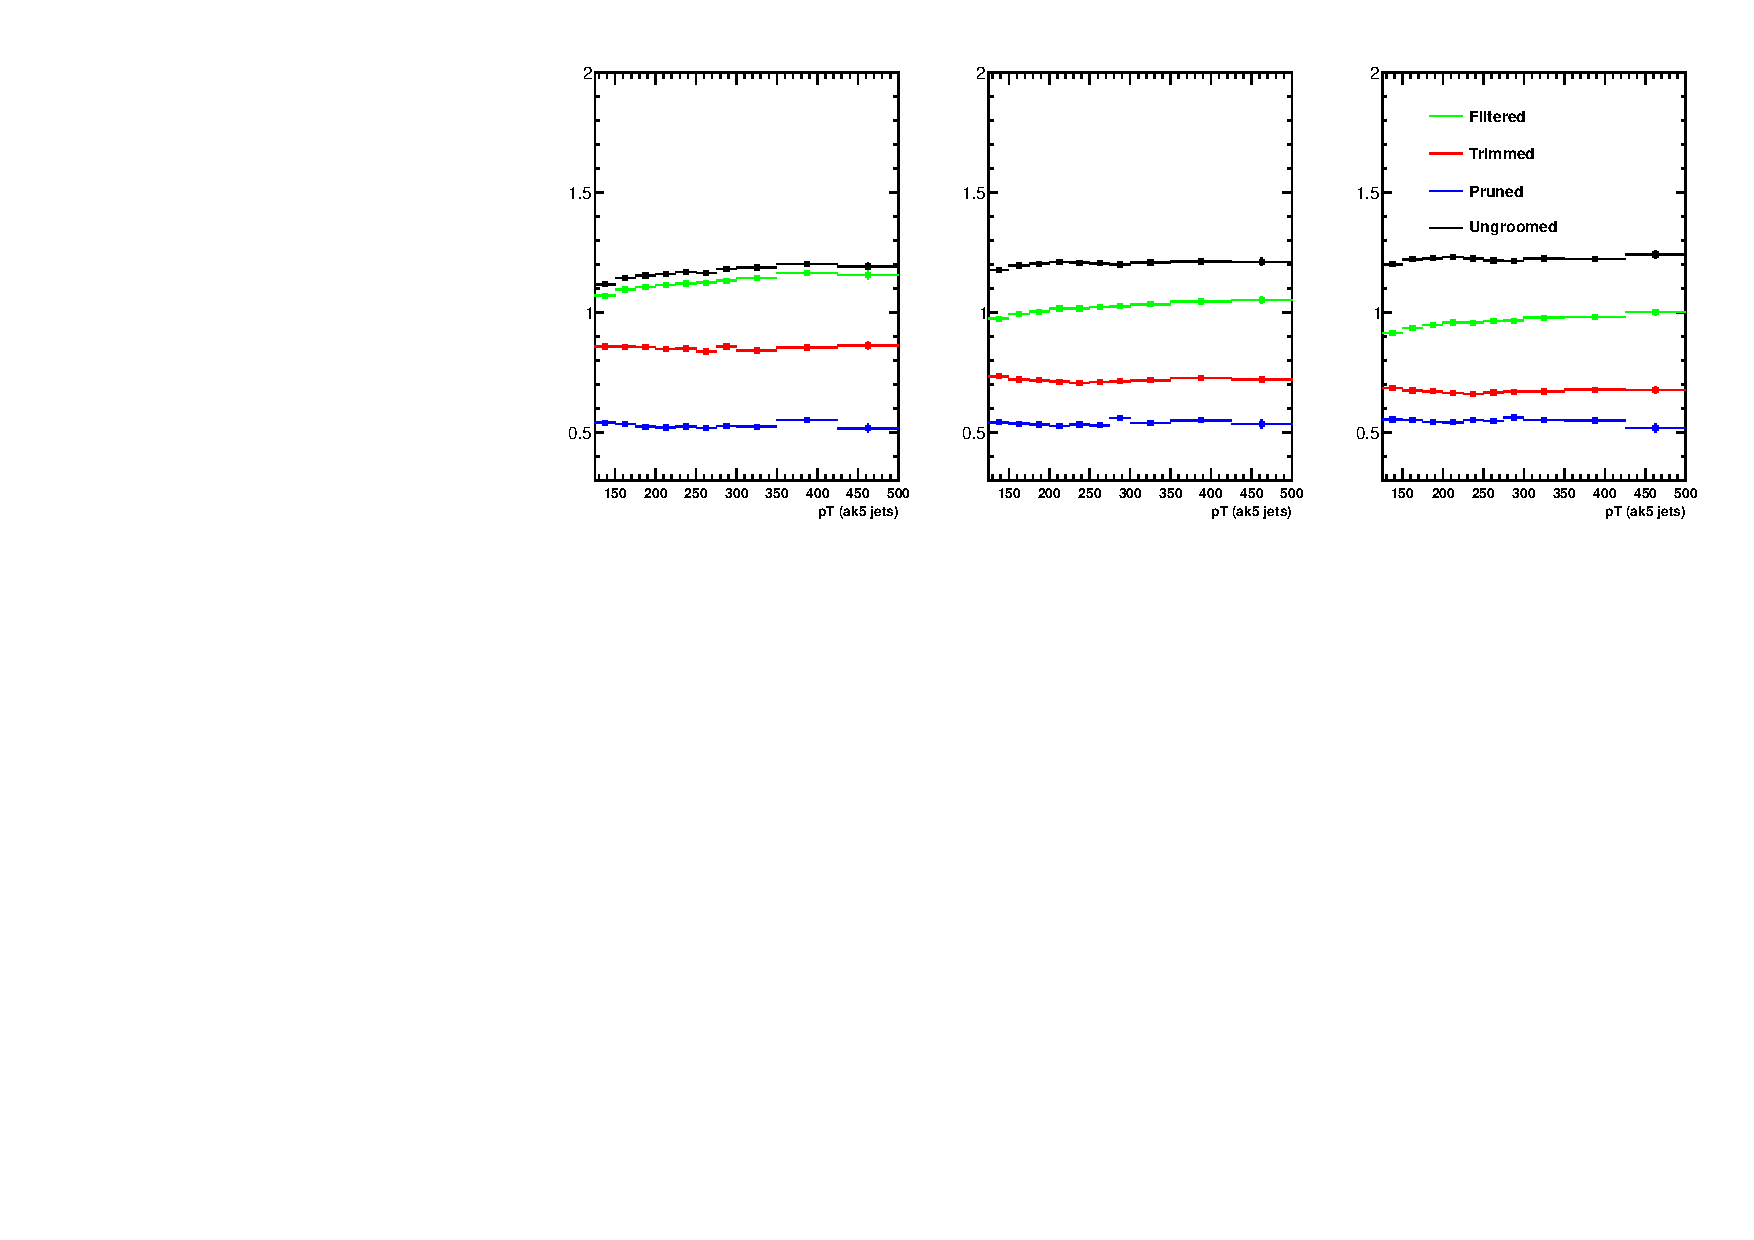
\includegraphics[width=1.0\textwidth]{figs/massRatioOvGen_vsPt.pdf}
\caption{Jet mass ratio for different jet algorithms as a function of the jet momentum. Here, the  substructure algorithms are compared to the
  generator-level AK5, AK7 and AK8 jets without the substructure algorithms applied.}
\label{figs:massRatio}
\end{figure}

We notice several interesting effects. First of all, we don't observe a sizable $p_t$ dependence for any of the ungroomed or groomed algorithms, apart for modest effect at low $p_t$  in the AK5 jets. In the ungroomed case, where we compare with ungroomed generator level jets, we see that the reconstructed mass overestimates the generated one by up to 20\%. This is not surprising and simply states that the reconstructed  mass has spurious constituents fromn the clustering process or PU residuals. The mass ratio for groomed jets becomes smaller and smaller the more aggressive the grooming is, up to the pruned jet where more than 40\% of the original ungroomed jet mass is removed by the pruning algorithm.  

Similar to the study above for the $p_T$ resolution, we then show the jet mass ratio  as a function of the jet pseudorapidity and the primary vertex multiplicity in fig.~\ref{figs:massRatiovsEta}-\ref{figs:massRatiovsNV}. No particular effect is seen in comparing the groomed jet behaviour with the ungroomed one.  

\begin{figure}[!htb]
\centering
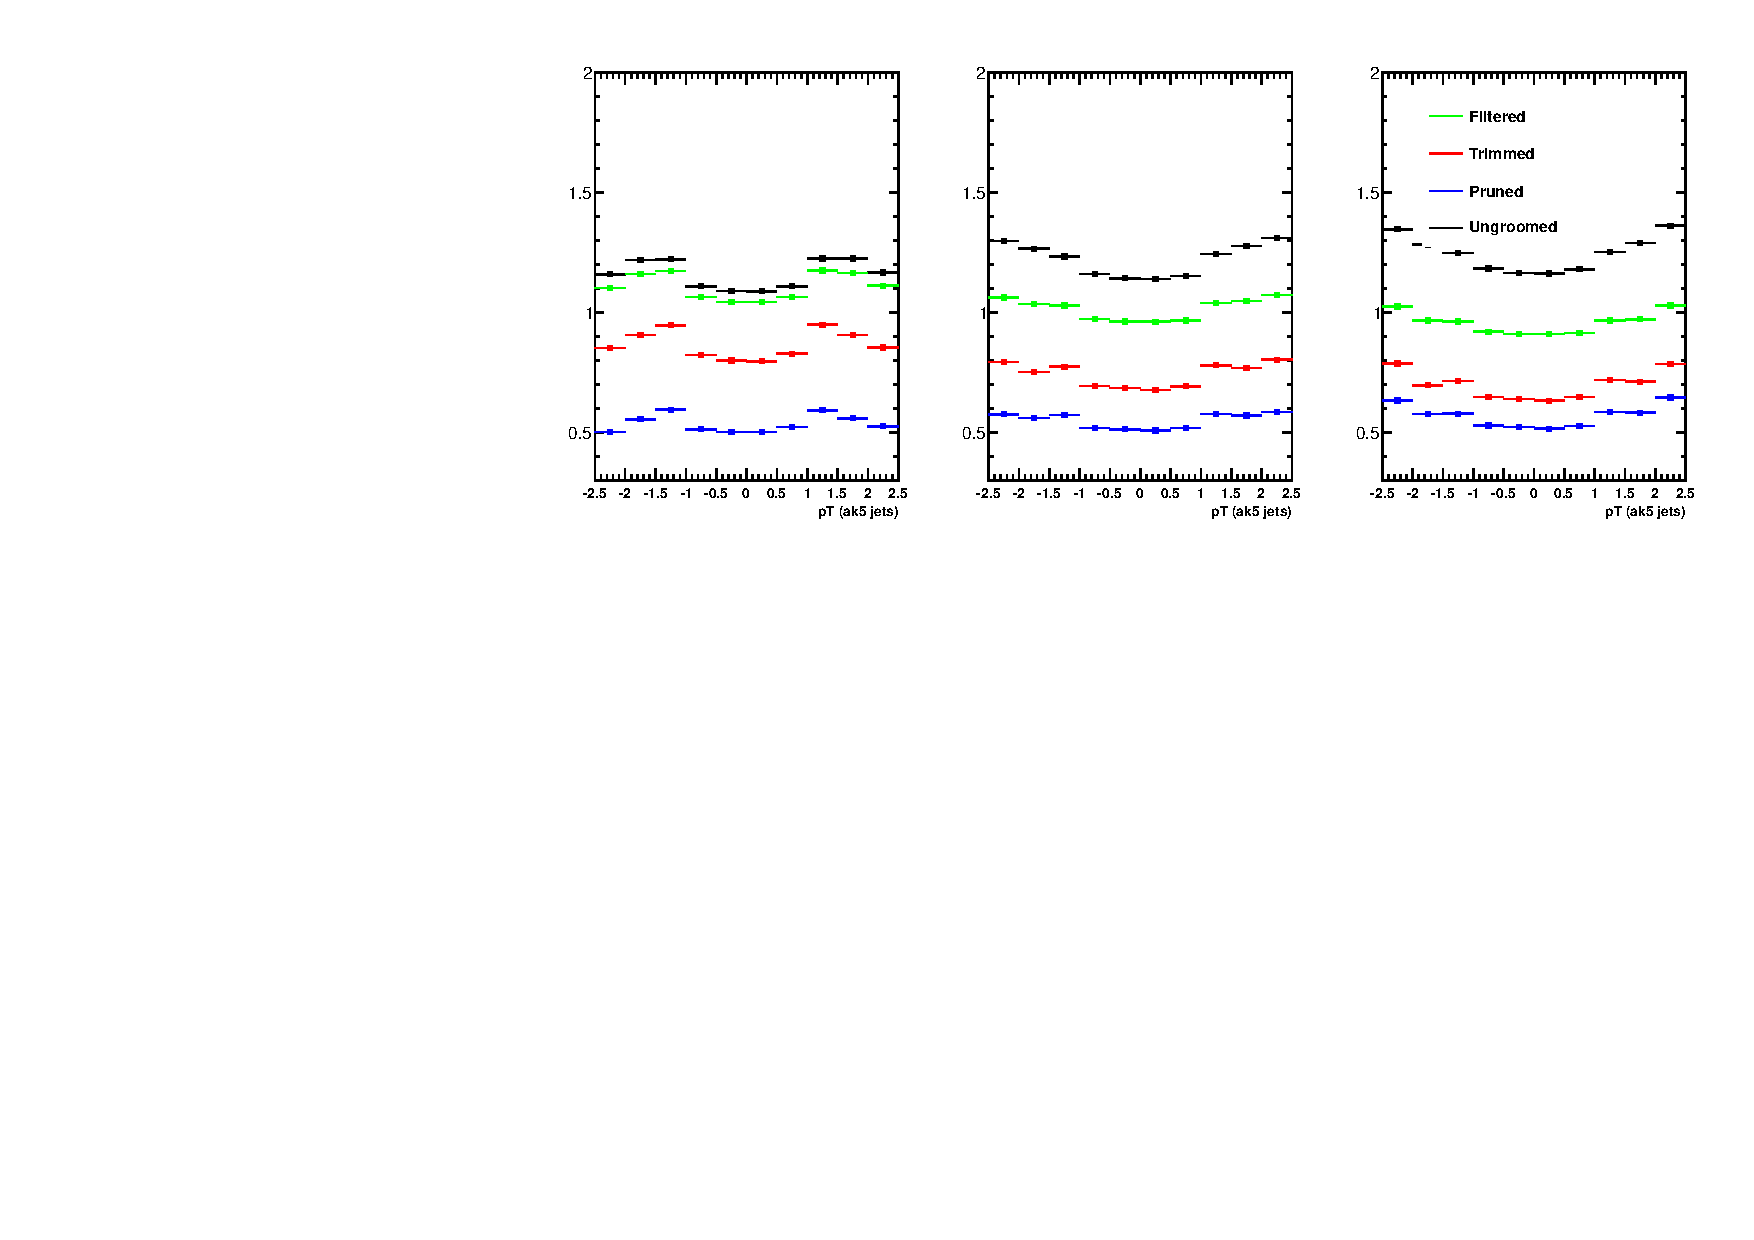
\includegraphics[width=1.0\textwidth]{figs/massRatioOvGen_vsEta.pdf}
\caption{Jet mass ratio for different jet algorithms as a function of the jet pseudorapidity. Here, the substructure algorithms are compared to the
  generator-level AK5, AK7 and AK8 jets without the substructure algorithms applied.}
\label{figs:massRatiovsEta}
\end{figure}

\begin{figure}[!htb]
\centering
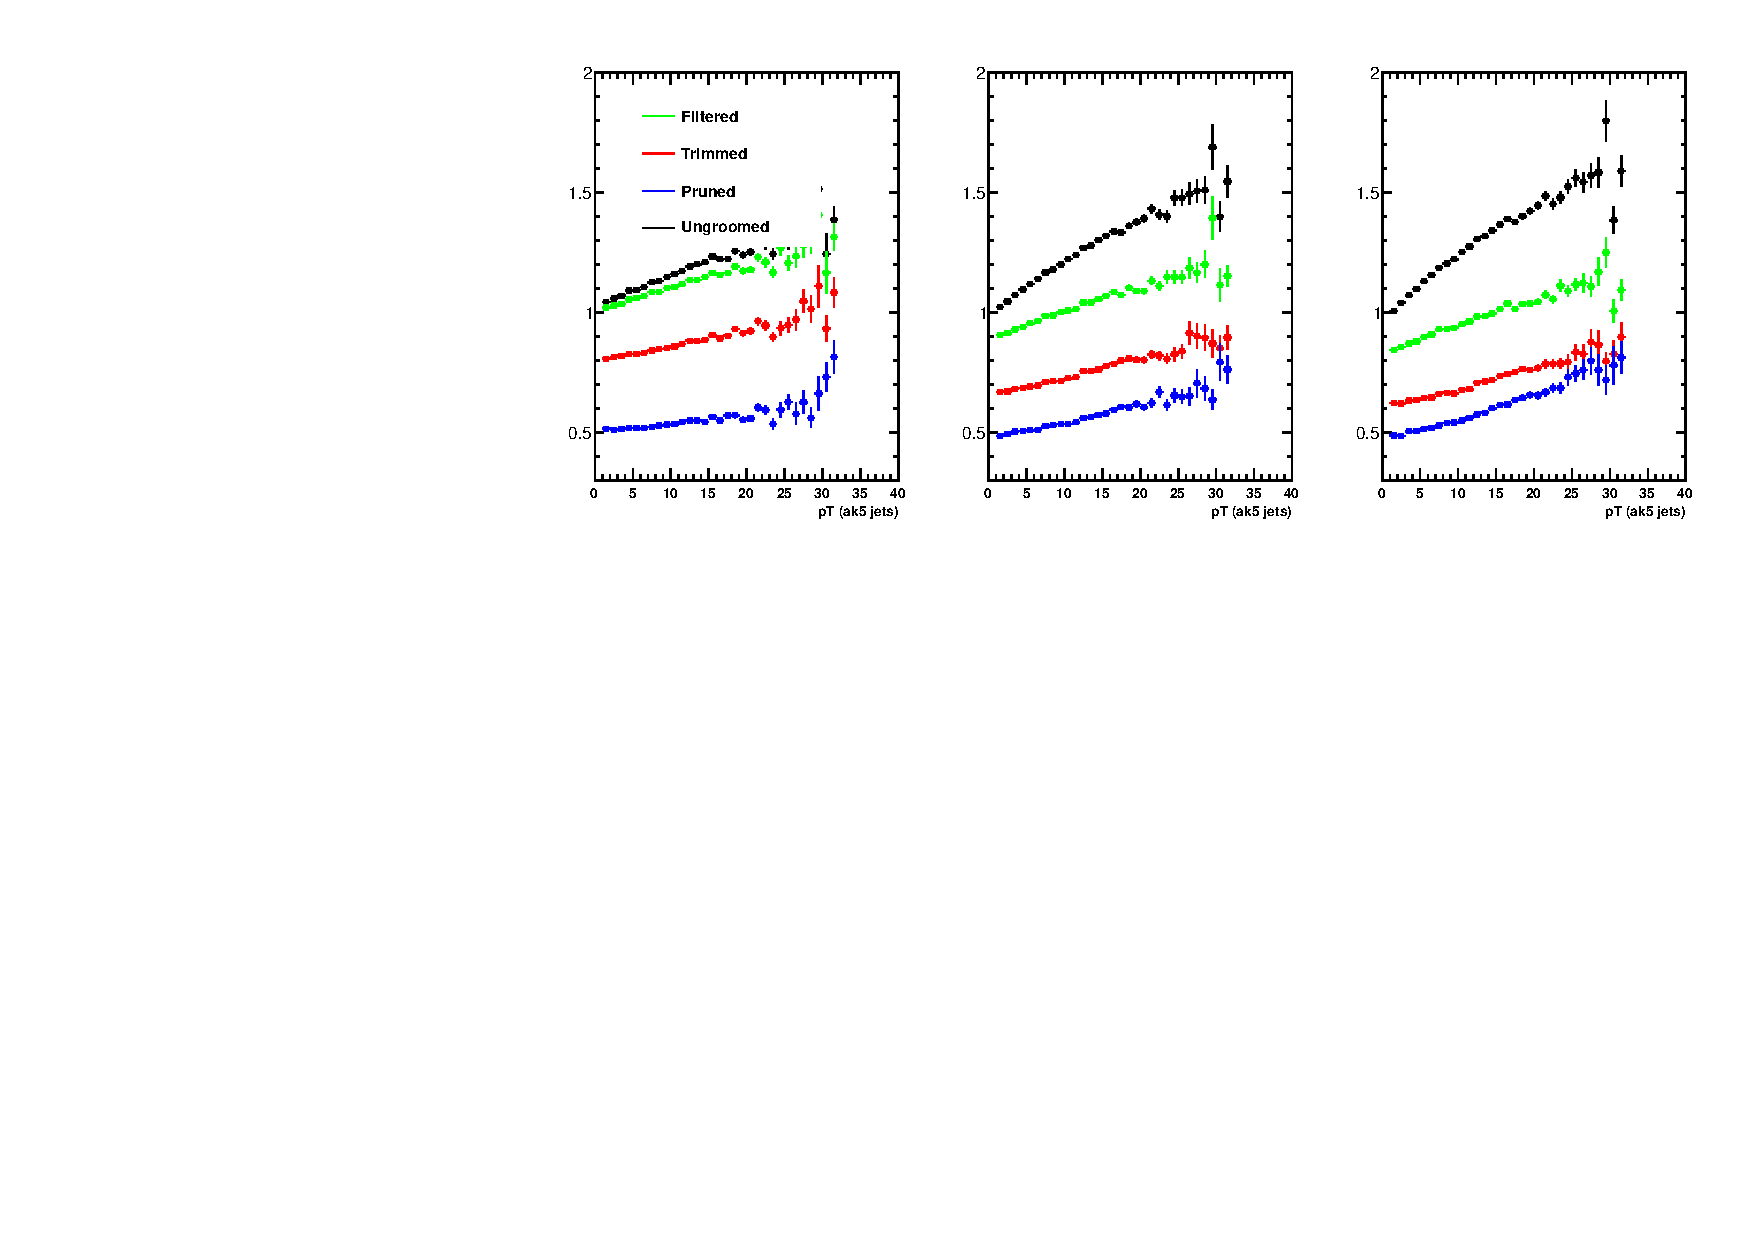
\includegraphics[width=1.0\textwidth]{figs/massRatioOvGen_vsNV.pdf}
\caption{Jet mass ratio for different jet algorithms as a function of the primary vertex multiplicity in the event. Here, the  substructure algorithms are compared to the
  generator-level AK5, AK7 and AK8 jets without the substructure algorithms applied.}
\label{figs:massRatiovsNV}
\end{figure}


In the jet mass ratio distributions considered so far we have compared the reconstructed (groomed or ungroomed) jet mass with the ungroomed generated one. We can now look at the same ratio using the reconstructed jet mass, i.e. measuring the ratio $(mass_{groomed} - mass_{ungroomed})/mass_{ungroomed}$. Fig.~\ref{figs:massRatioData} shows this ratio as a function of the jet momentum in data and MC events.

\begin{figure}[!htb]
\centering
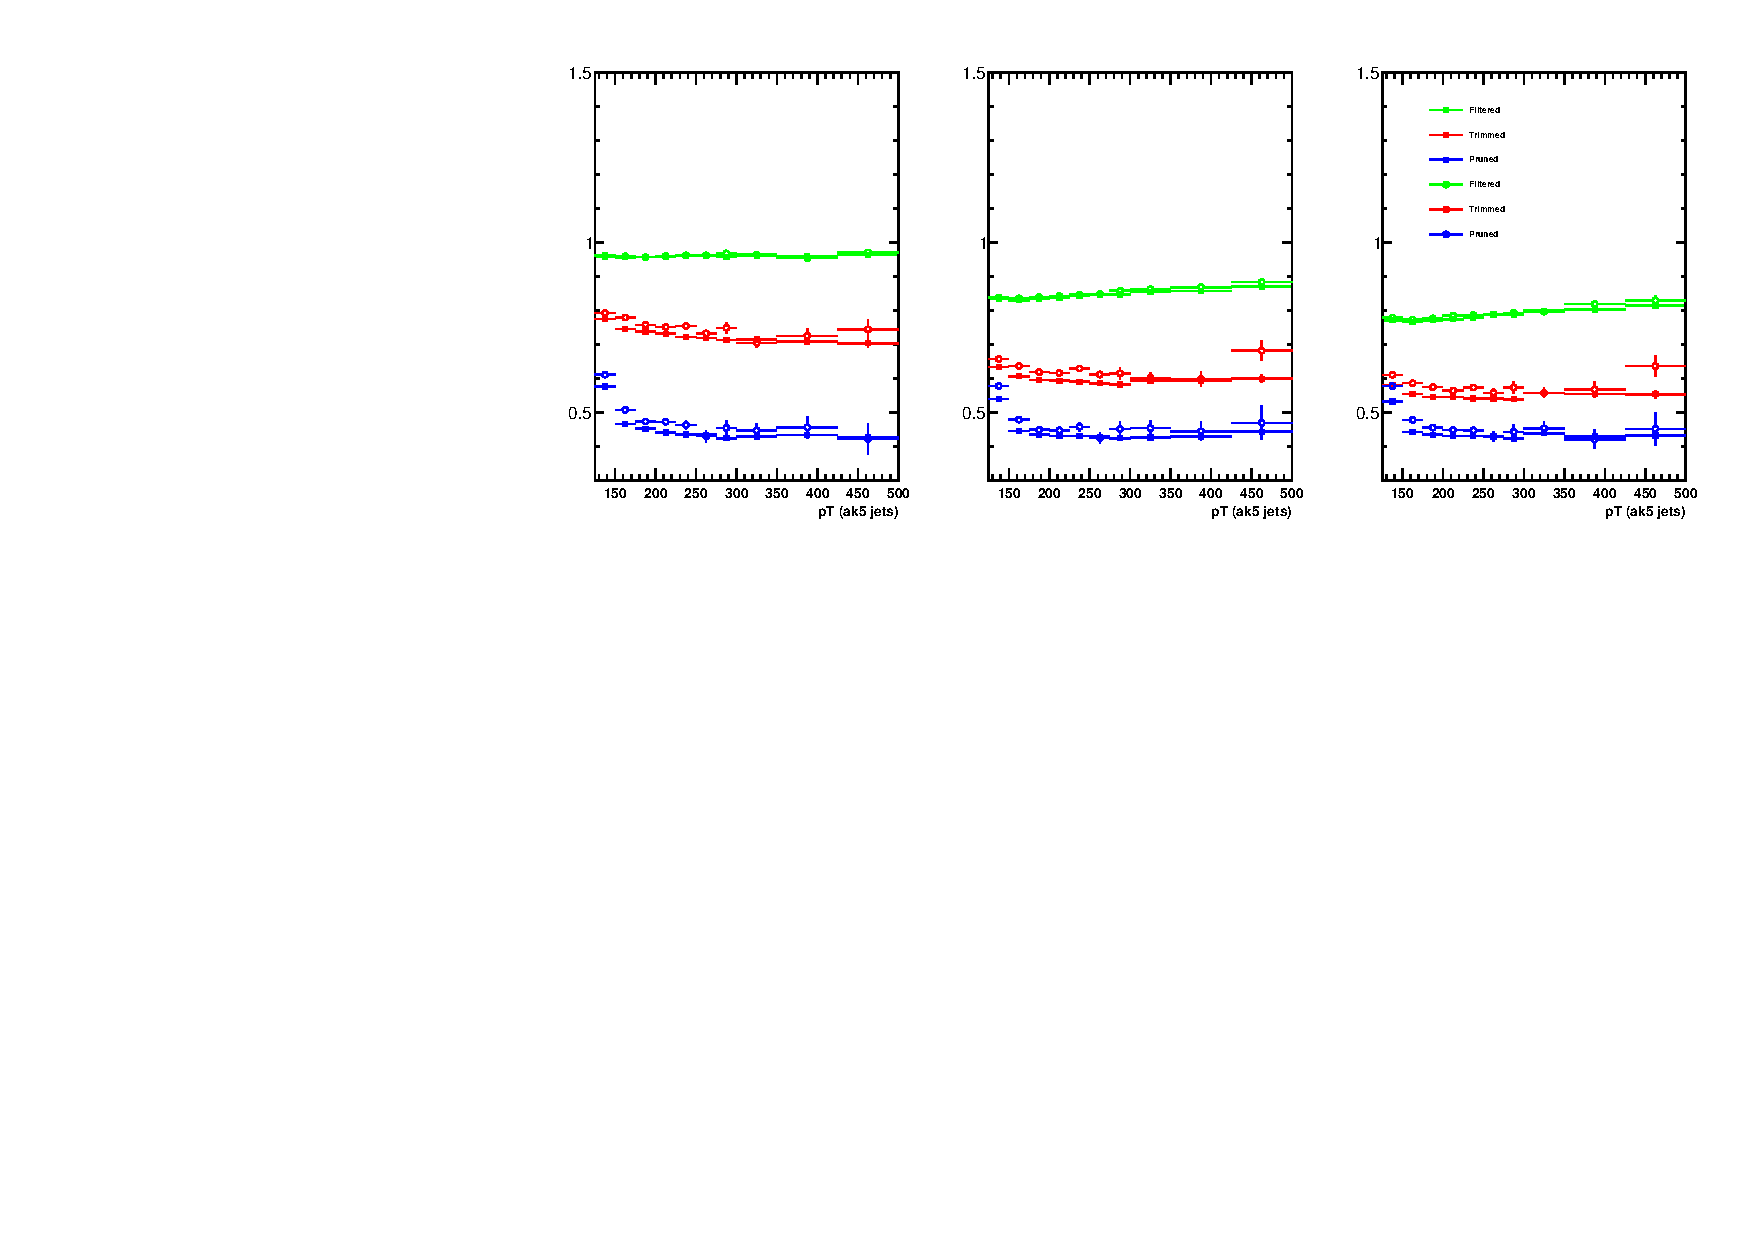
\includegraphics[width=1.0\textwidth]
{figs/massRatioOvReco_vsPt.pdf}
\caption{Reconstructed Jet mass ratio for different jet algorithms as a function of the jet momentum. 
Here, the substructure algorithms are compared to the
  reconstructed ungroomed AK5, AK7 and AK8 jets. Data: empty cicle, MC: filled square.}
\label{figs:massRatioData}
\end{figure}
     
The 1-d distribution for the jet mass ratio is shown in Fig.~\ref{figs:1dJetMassRatio}. In this plot we show the ratio of the different AK7 ungroomed algorithm w.r.t. ungroomed jets. For data and MC we show this ratio for reconstructed jets, while for the MC we also show the same ratio for the generated jet mass.   

\begin{figure}[!htb]
\centering
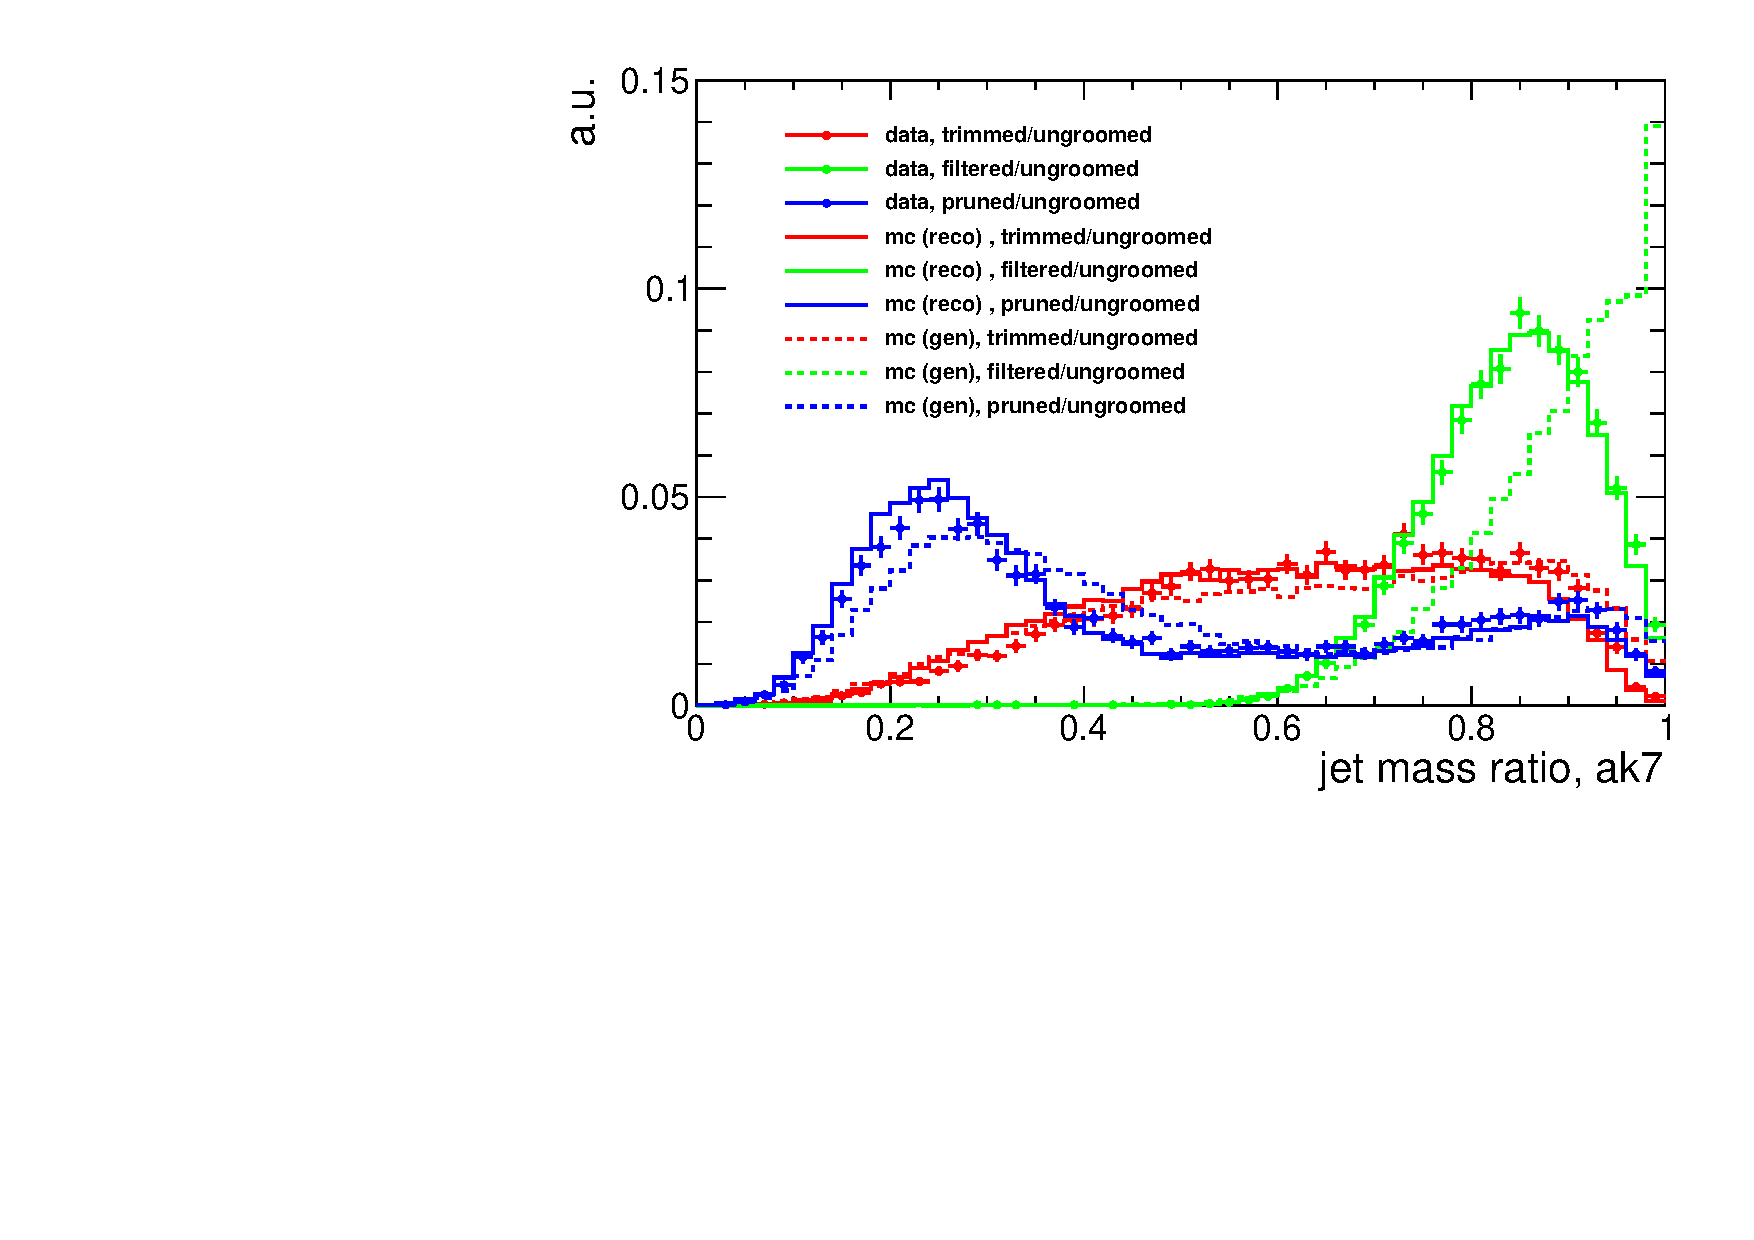
\includegraphics[width=1.0\textwidth]{figs/jetmass_1Dratio_ak7.pdf}
\caption{Reconstructed Jet mass ratio for different jet algorithms. The substructure algorithms are compared to the
  reconstructed AK7 jets.}
\label{figs:1dJetMassRatio}
\end{figure}


\subsection{TTbar Control sample}

As an additional check on the performance of the grooming algorithms, and a direct estimate of (any) data/MC difference in the algorithm efficiency, we can build a $t\bar{t}$ control sample in $W(\mu\nu)$ and $W(e\nu)$ + jet events. An enriched $t\bar{t}$ control sample can easily be obtained by requiring additional jet activity in the event, defined as additional AK5 jets  in the event that are not within a certain $\Delta R$ of the leading boosted jet, and with at least one of these jet passing a tight $b$-tagging requirement.

For CA8 pruned jets, due to the jet clustering radius, the leading jet in $t\bar{t}$ events will likely be the $W$ from the top hadronic decay ($t \to W(jj)b$). A clean peak in the jet mass distributiobn for CA8 pruned jet is obtained by requiring the jet $p_T >200$ GeV and a significant mass drop ($<0.3$), as shown in Fig.~\ref{figs:Wtagging08}.

\begin{figure}[!htb]
\centering
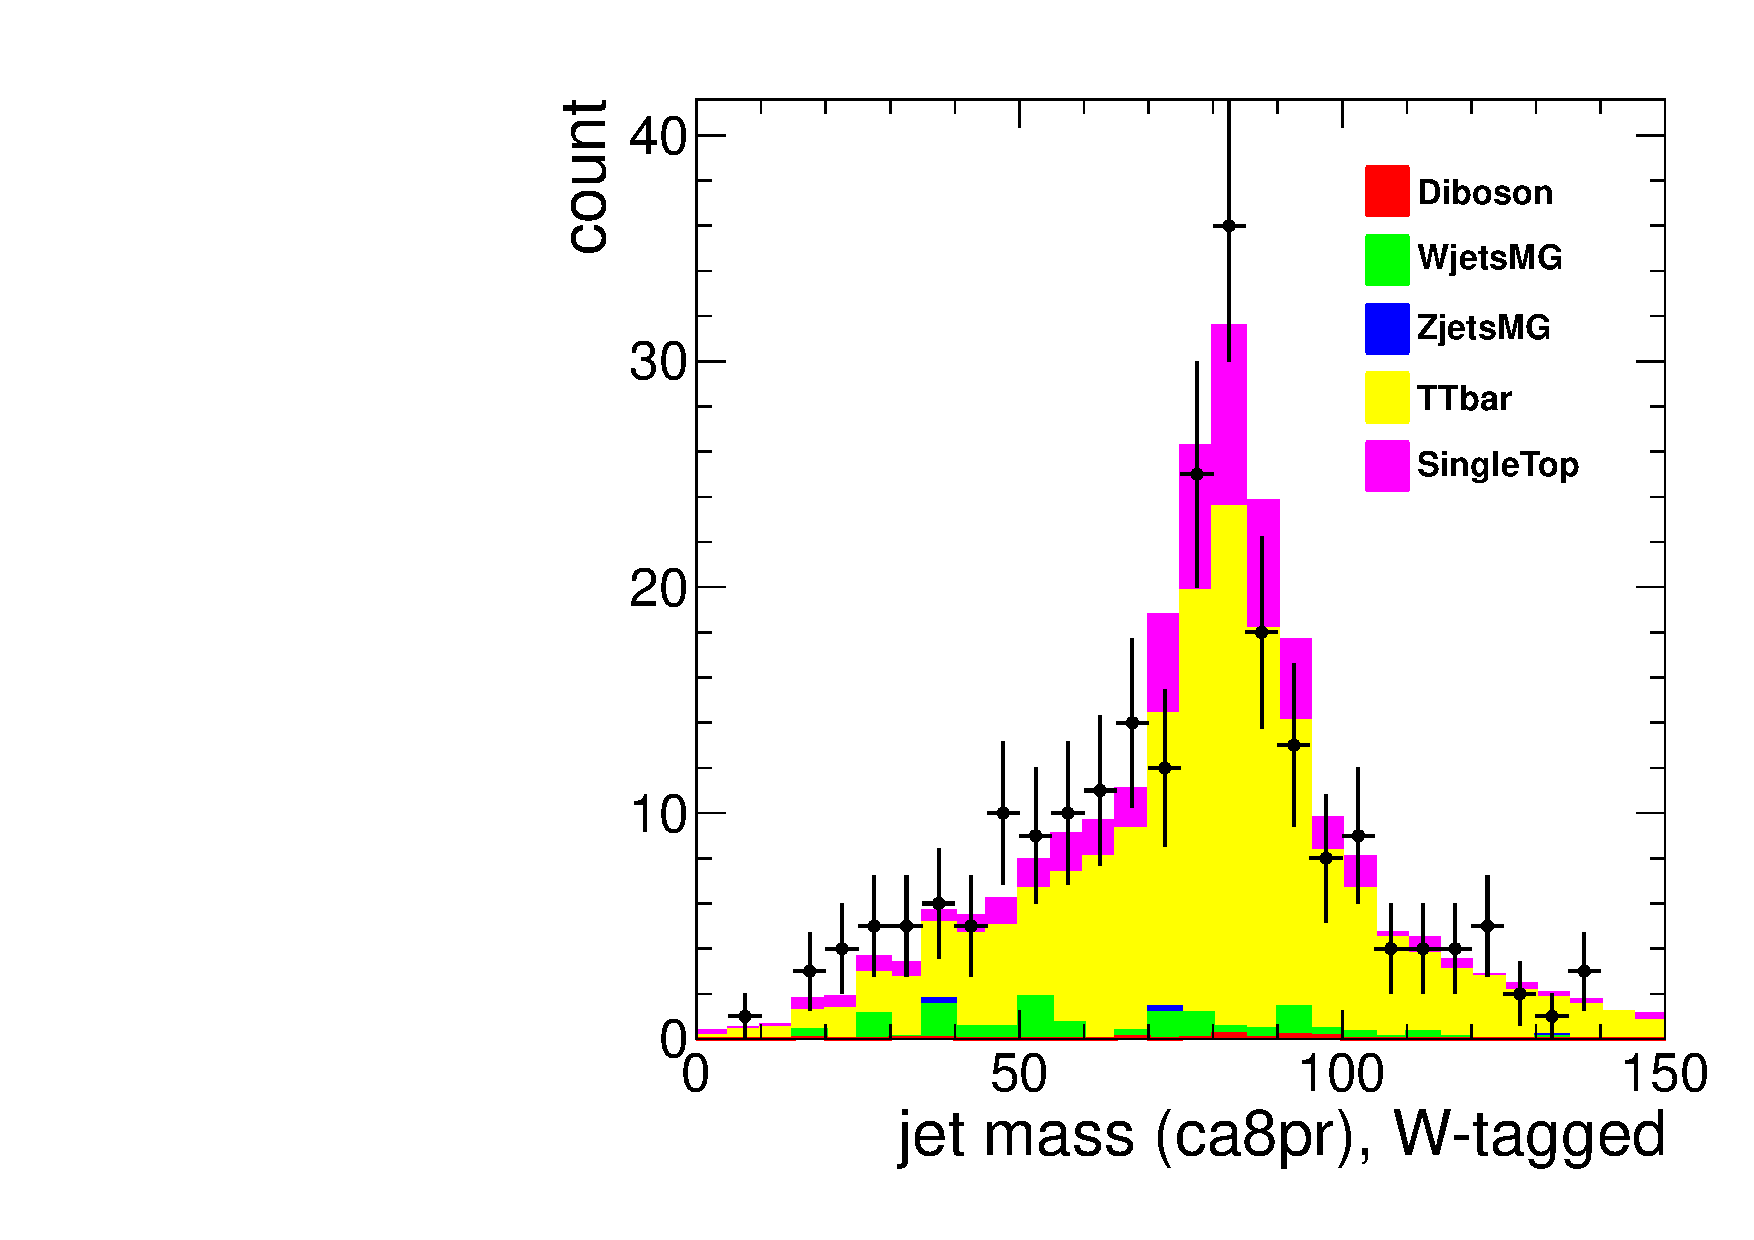
\includegraphics[width=0.49\textwidth]{figs/Wen/taggedW_ca8pr.pdf}
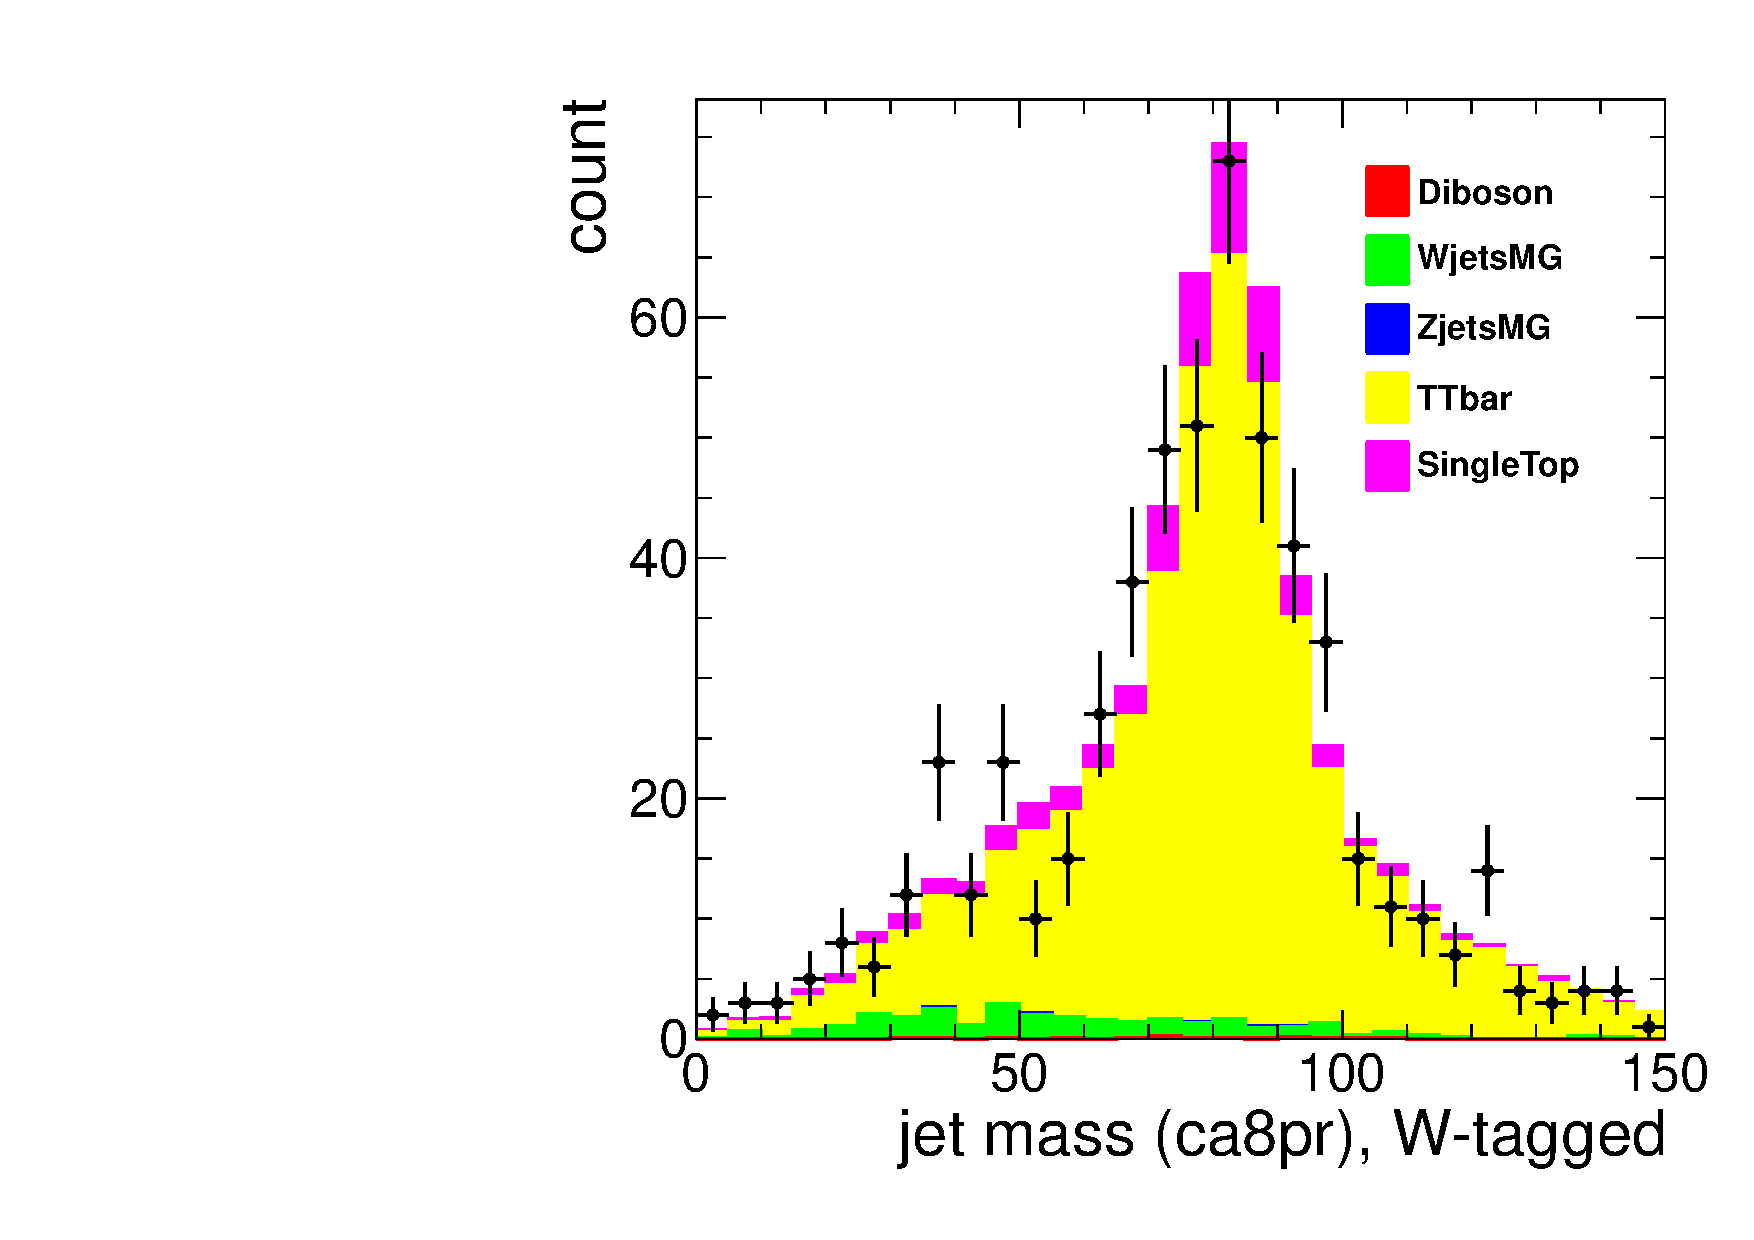
\includegraphics[width=0.49\textwidth]{figs/Wmn/taggedW_ca8pr.pdf}
\caption{$W$ tagging for CA8 pruned jet in a $t\bar{t}$ data control sample. The data (points with error bars) is compared tostacked sum of MC contributions. The MC is normalized to the data integral. Left: electron sample, right: muon sample.}
\label{figs:Wtagging08}
\end{figure}
  
For C1A12 jet, due to the jet clustering radius, the leading jet could either contain the full hadronic top decay, or just the hadronic W decay. We identify top fully reconstructed within the CA12 jet by requiring three filtered jet with $p_T>30$ FGeV, while we identify hadronic $W$ decays by requiring only two filtered jets with $p_T > $30 GeV, and the third one (if present) below $20$ GeV.

Fig.~\ref{figs:Wtagging12} shows the CA12 filtered jet mass for events in the $t\bar{t}$ control sample passing the $W$-tagging cuts, while Fig.~\ref{figs:toptagging12} shows the jet mass for events passing the top-tagging selection.

\begin{figure}[!htb]
\centering
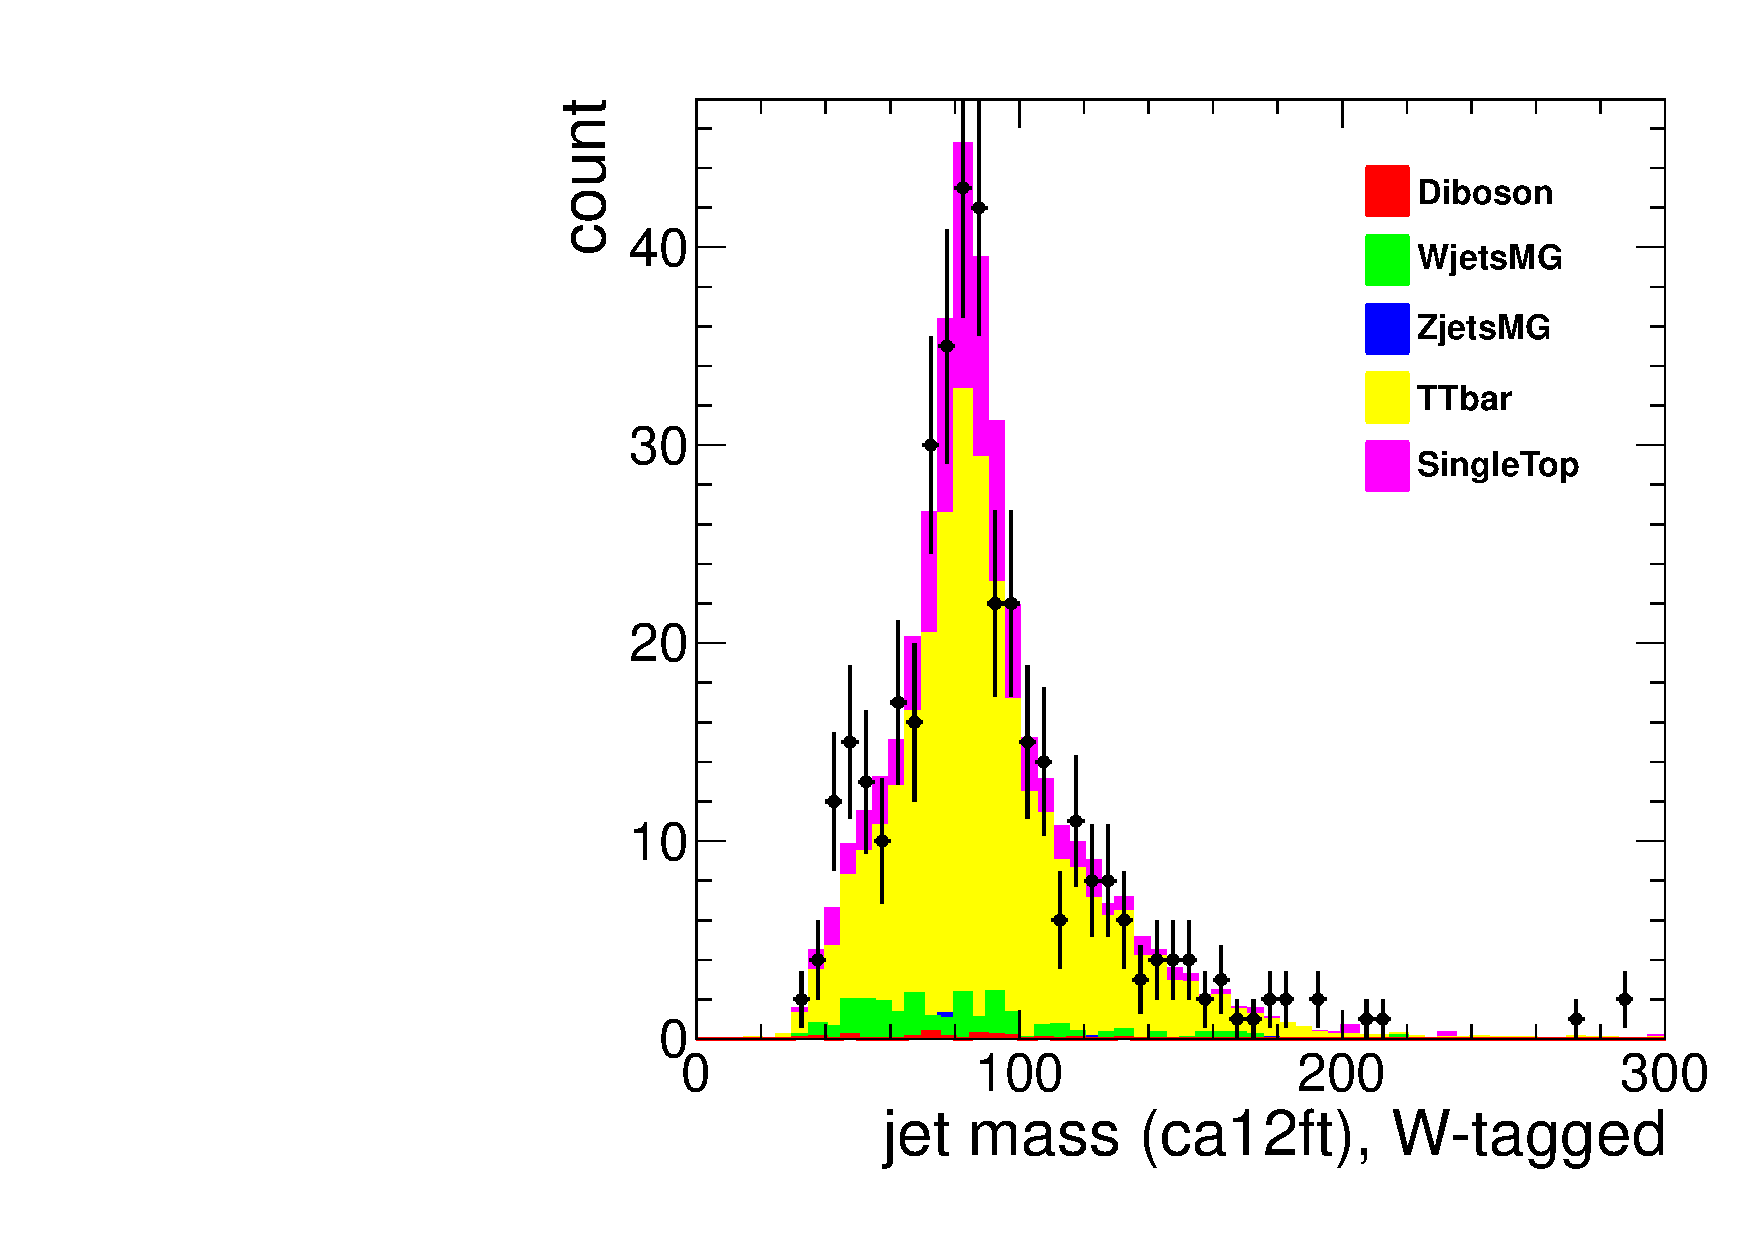
\includegraphics[width=0.49\textwidth]{figs/Wen/taggedW_ca12ft.pdf}
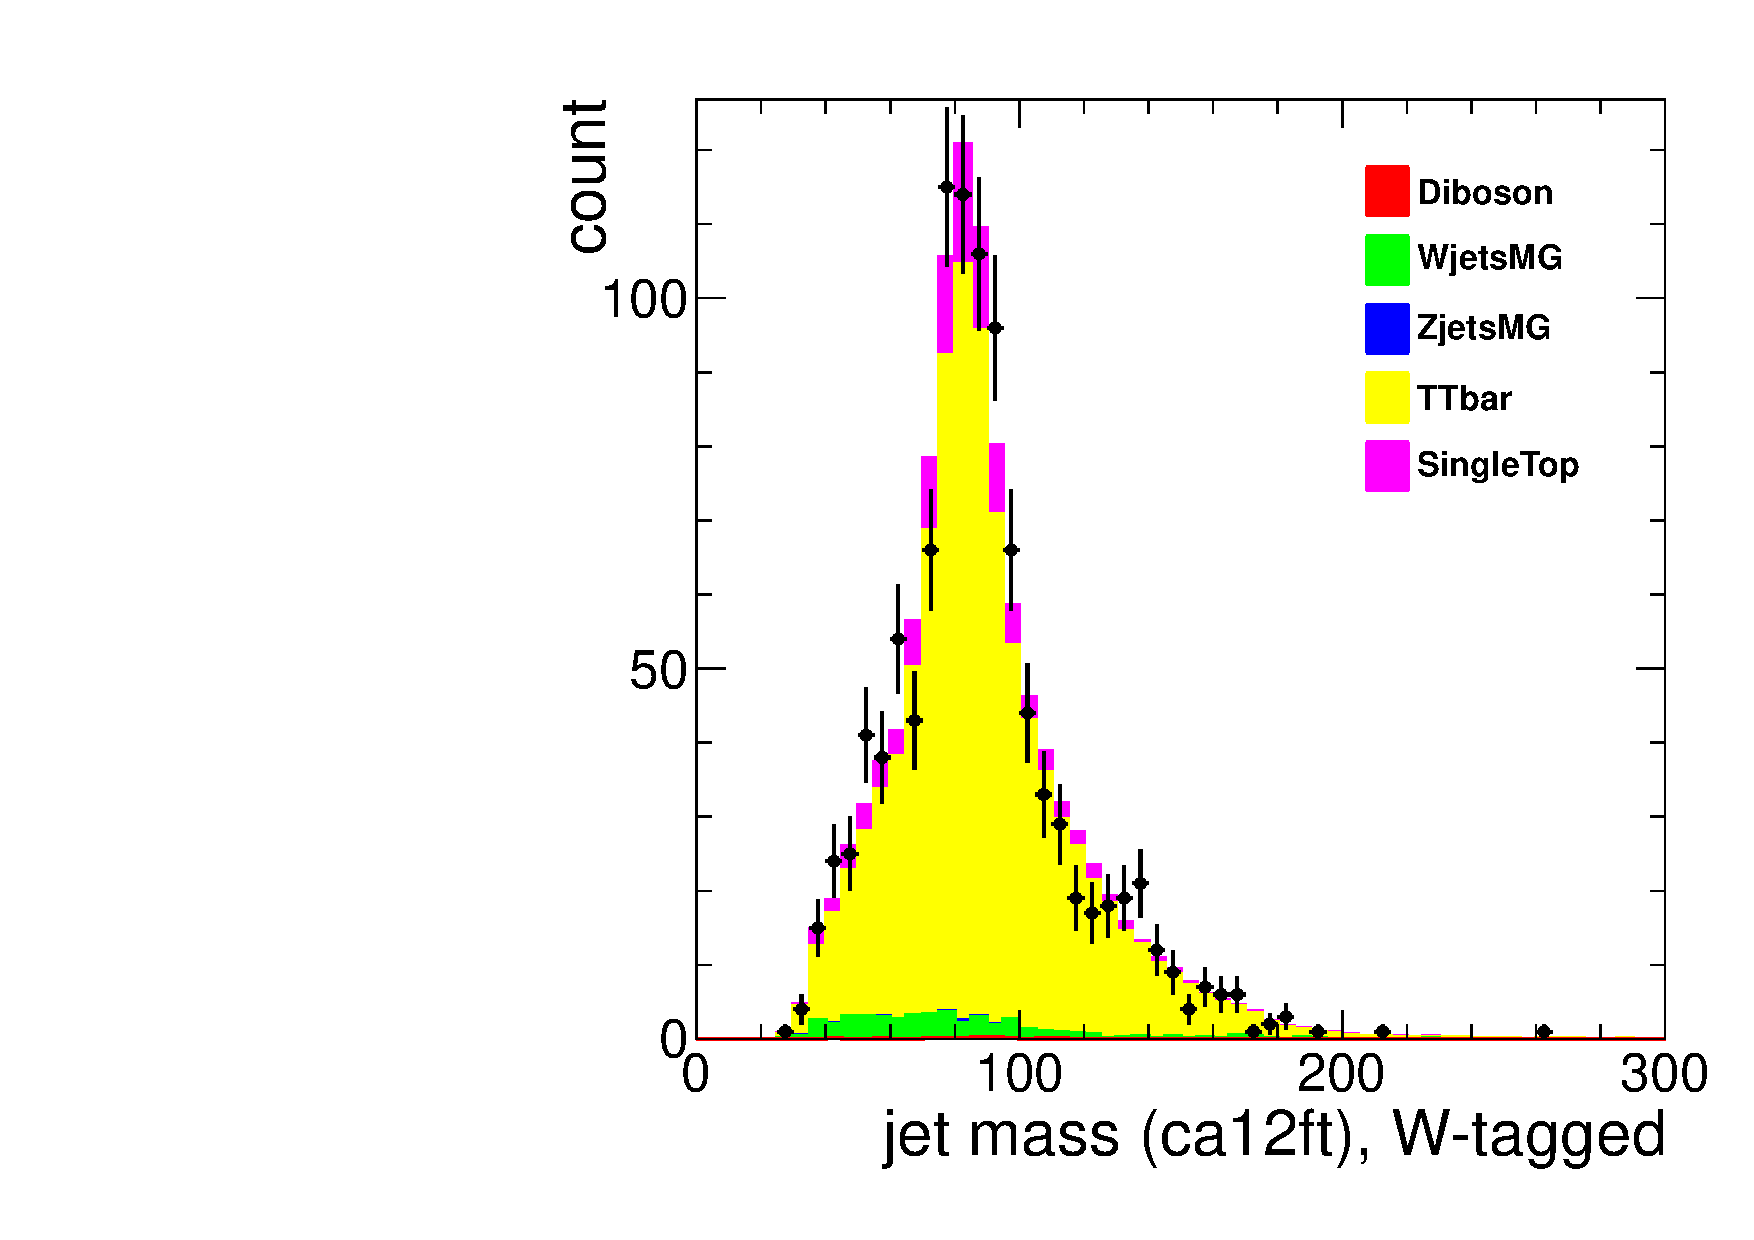
\includegraphics[width=0.49\textwidth]{figs/Wmn/taggedW_ca12ft.pdf}
\caption{$W$ tagging for CA12 filtered jet in a $t\bar{t}$ data control sample. The data (points with error bars) is compared tostacked sum of MC contributions. The MC is normalized to the data integral. Left: electron sample, right: muon sample.}
\label{figs:Wtagging12}
\end{figure}

\begin{figure}[!htb]
\centering
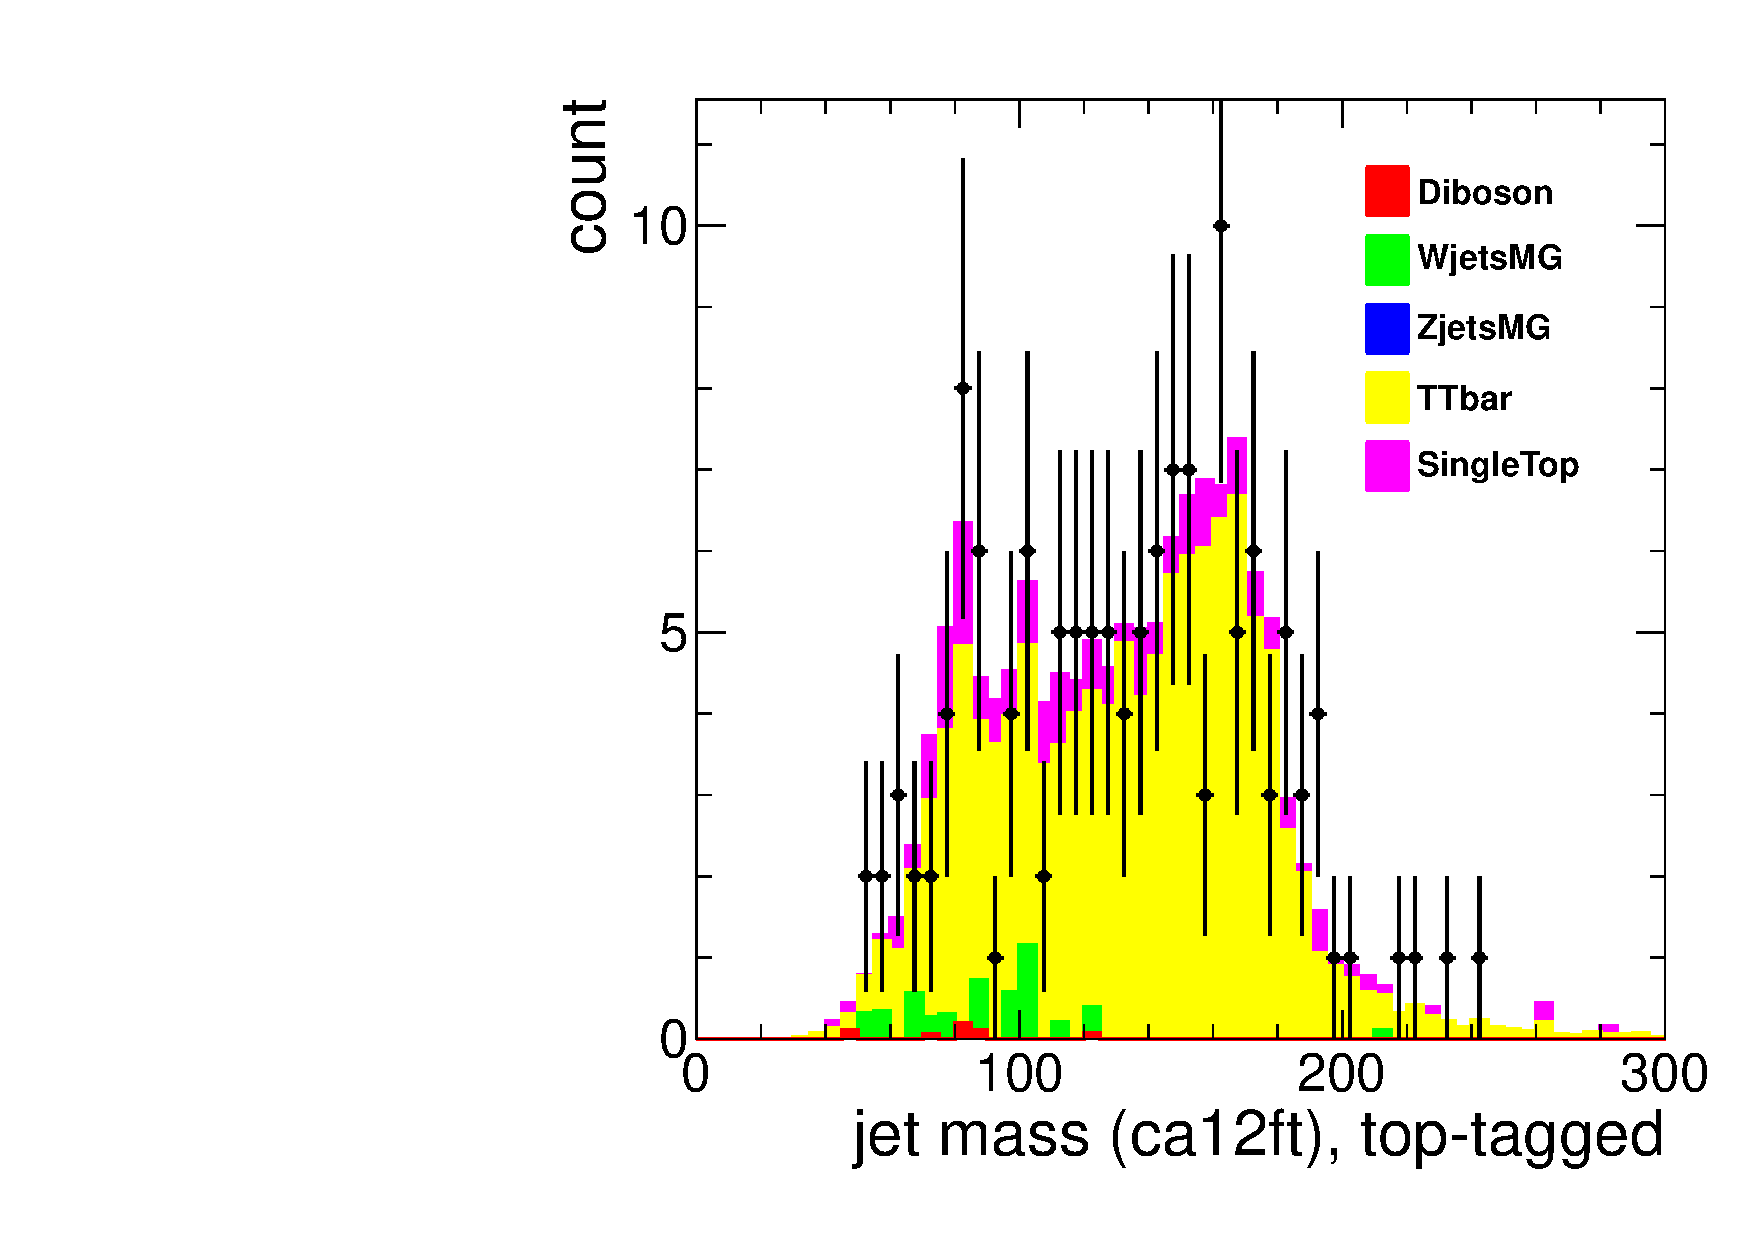
\includegraphics[width=0.49\textwidth]{figs/Wen/taggedTop_ca12ft.pdf}
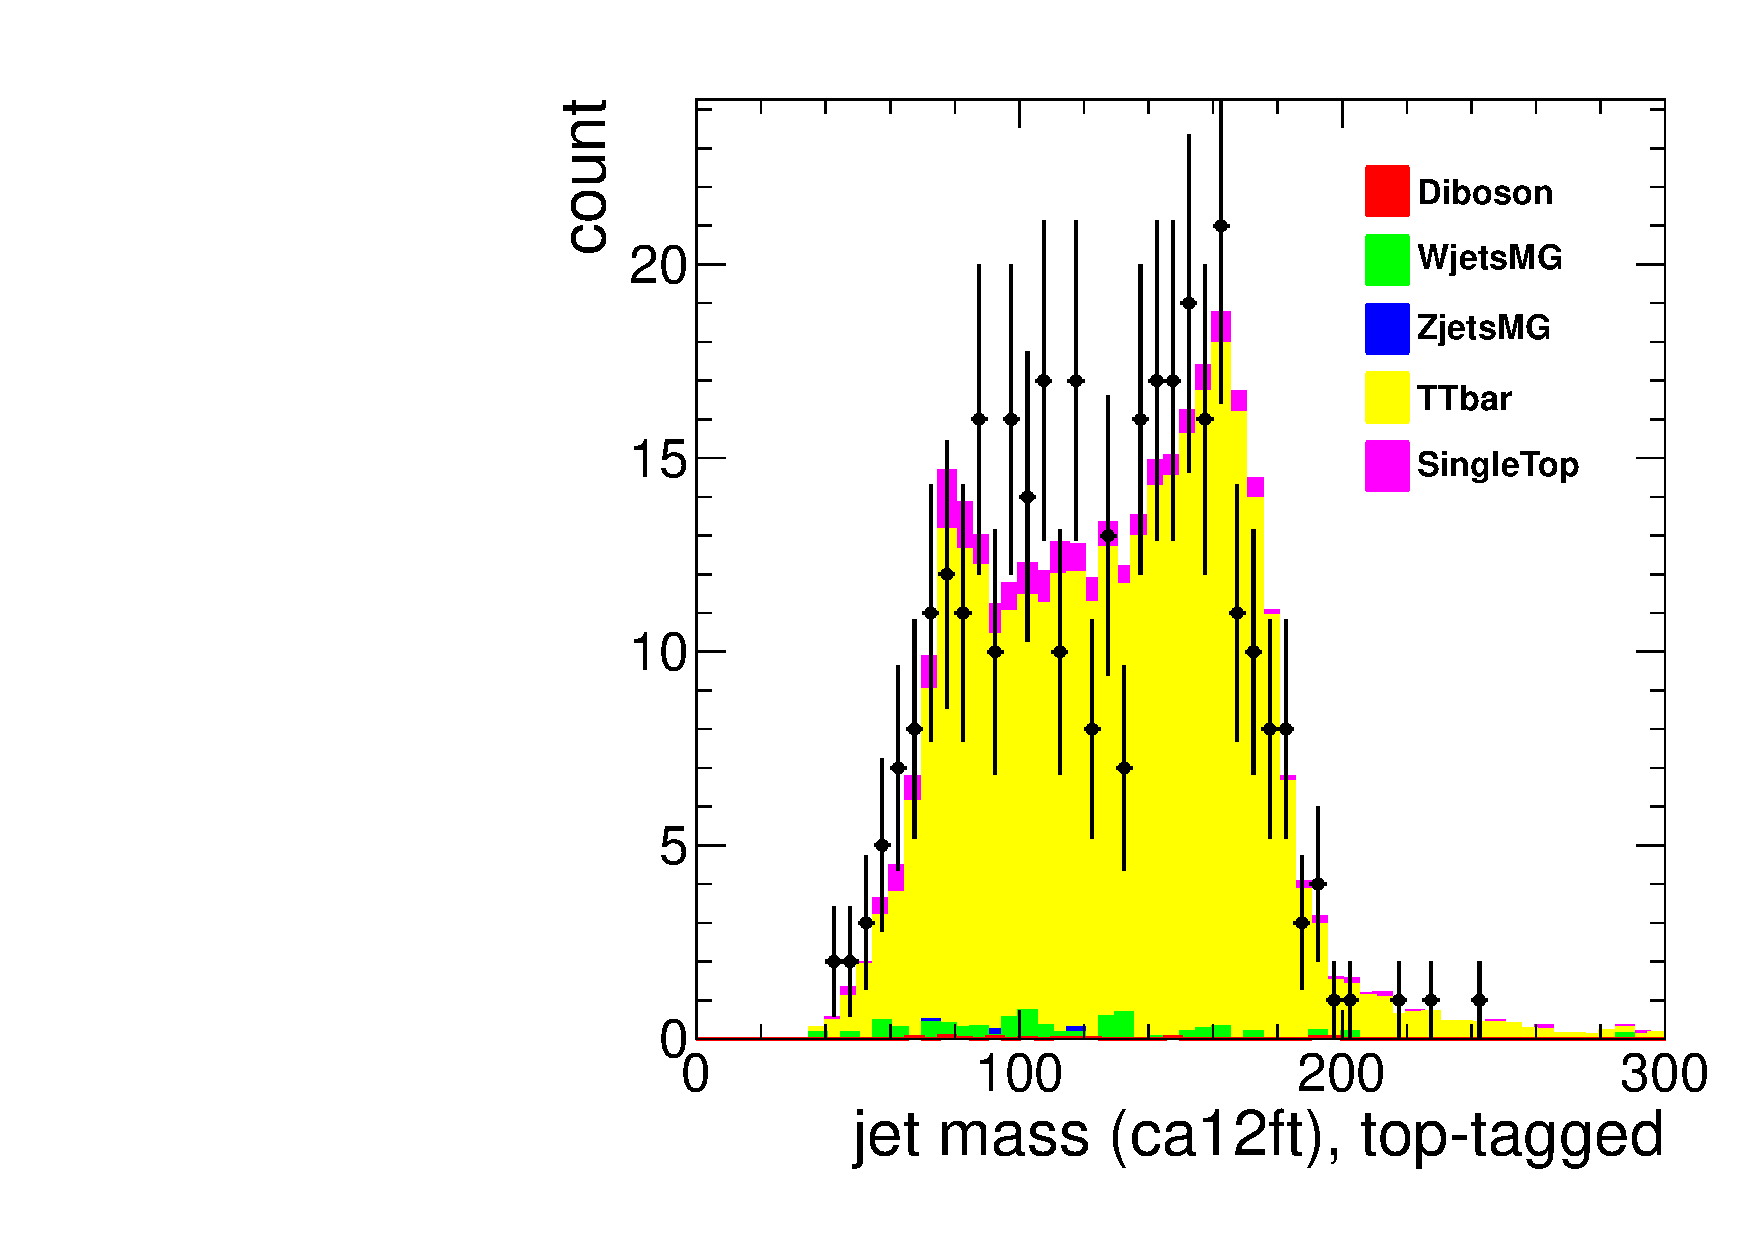
\includegraphics[width=0.49\textwidth]{figs/Wmn/taggedTop_ca12ft.pdf}
\caption{Top-tagging for CA12 filtered jet in a $t\bar{t}$ data control sample. The data (points with error bars) is compared tostacked sum of MC contributions. The MC is normalized to the data integral. Left: electron sample, right: muon sample.}
\label{figs:toptagging12}
\end{figure}
 
In all cases, the MC nicely reproduces the jet mass distribution obtained on data.

%that have the same substructure algorithm applied as the reconstructed-level
%jets. That is, \verb!AK5PFJets! are compared to \verb!AK5GenJets! in both
%plots, \verb!CA8PFJets! are compared to \verb!CA8GenJets! in both plots,
%\verb!CA8PFJets! with top tagging are compared to \verb!CA8GenJets! with
t%op tagging, and \verb!CA8PFJets! with pruning are compared to \verb!CA8GenJets!
%with pruning. The top tagged jets (in purple) are directly above the ``bare''
%CA8 jets, because the algorithm does not modify the total jet.

% This shows us
%that the AK5 jet corrections are working as expected for the CA8 jets.
%The conservative 3\% systematic uncertainty we are applying in addition to the
%default uncertainties covers this effect.

%However, if the same procedure is applied to the generator-level jets,
%the agreement is much better, with a bias of 2\%. This means that the jet
%pruning algorithm is slightly more aggressive in the ``simulated data''
%than it is at the generator particle level.



\fi



